\chapter{Gallery}

This chapter showcases some test cases that have been performed with PSD.

\begin{figure}
    \centering
    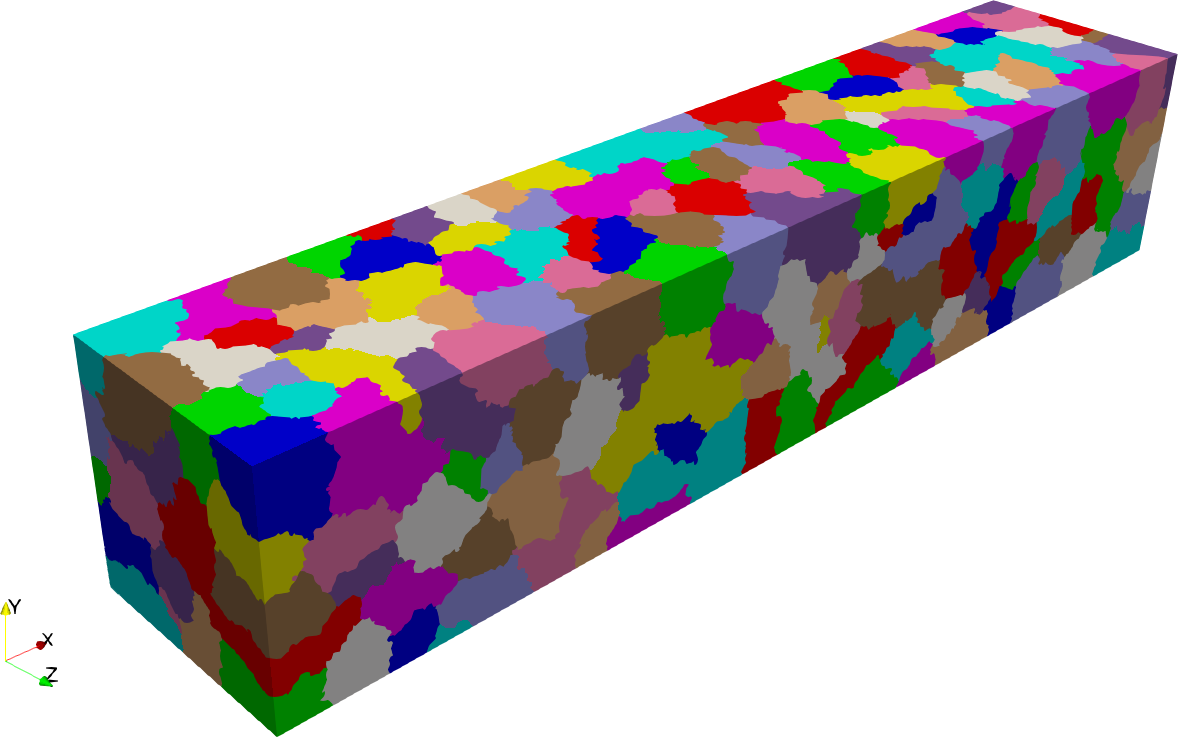
\includegraphics[width=0.5\textwidth]{./Images/400partmesh3d.png}
    \caption{90 M dof with 400 partitions.}
    \label{fig:90Mdof}
\end{figure}


\begin{figure}
	\centering
	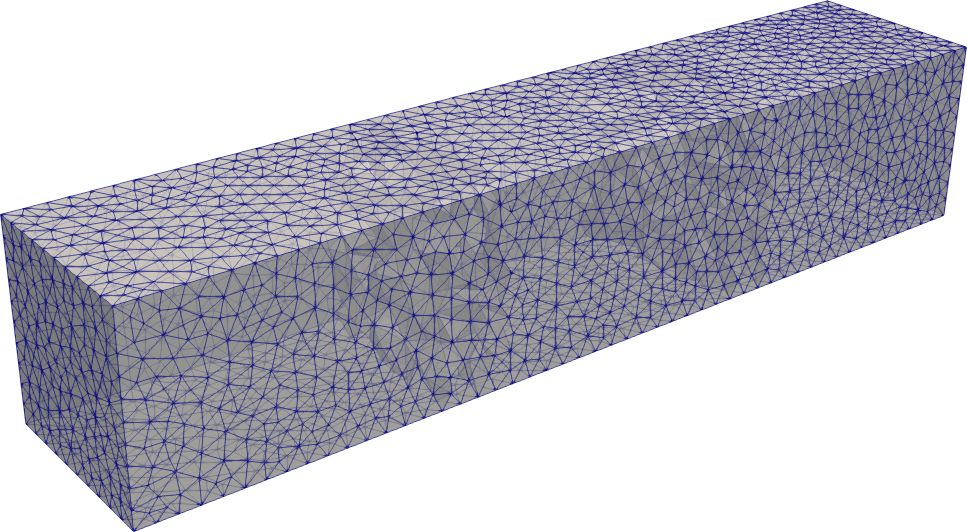
\includegraphics[width=0.45\textwidth]{./Images/bar-1.png}    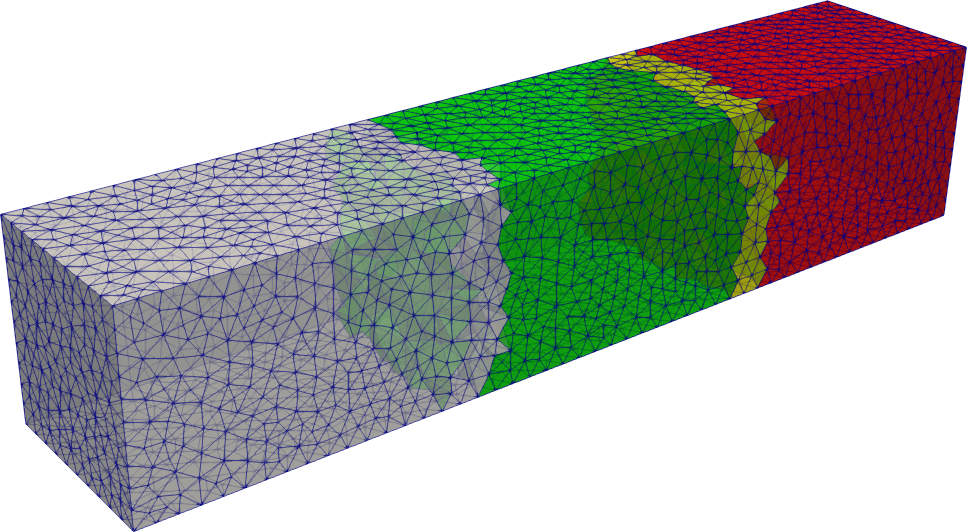
\includegraphics[width=0.45\textwidth]{./Images/bar-2.png}\\
	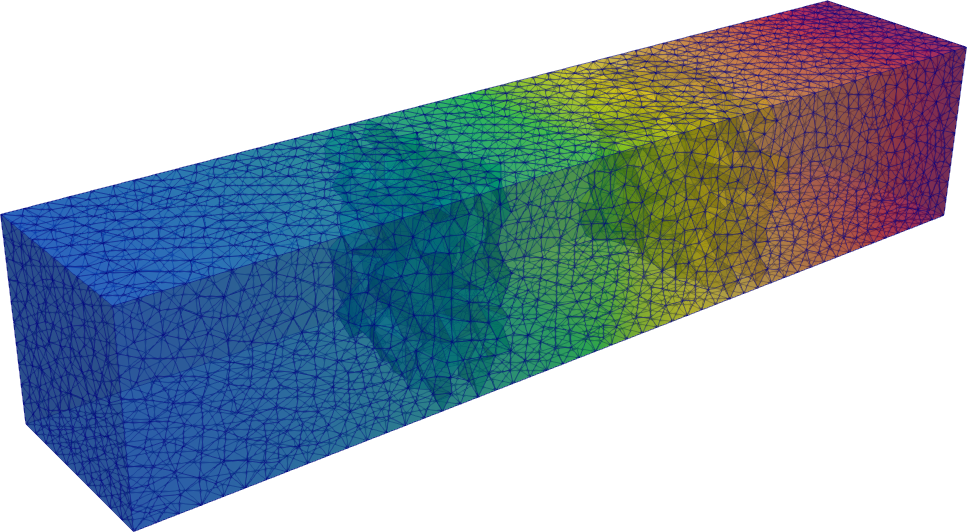
\includegraphics[width=0.45\textwidth]{./Images/bar-3.png}
	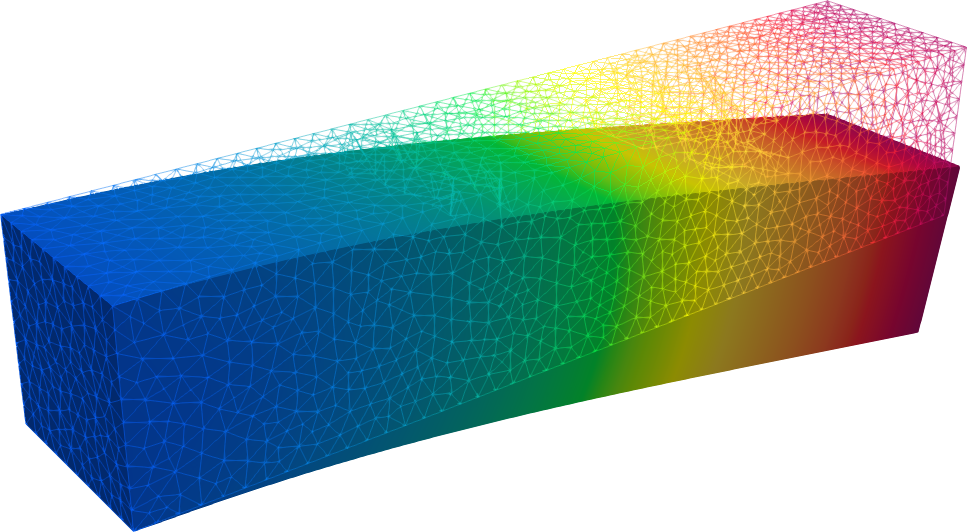
\includegraphics[width=0.45\textwidth]{./Images/bar-4.png}
	\caption{Bending of clamped bar under loading.}
	\label{fig:bar}
\end{figure}

\begin{figure}
    \centering
    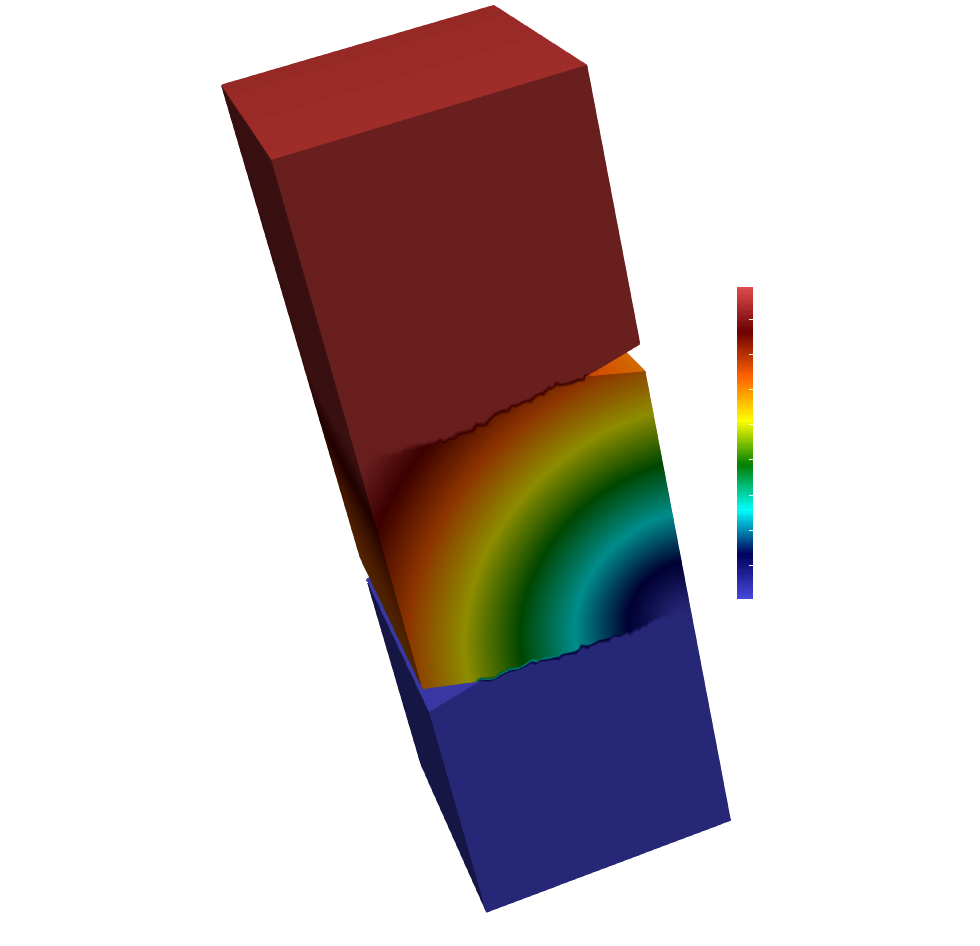
\includegraphics[width=0.45\textwidth]{./Images/rainbow-test.png}    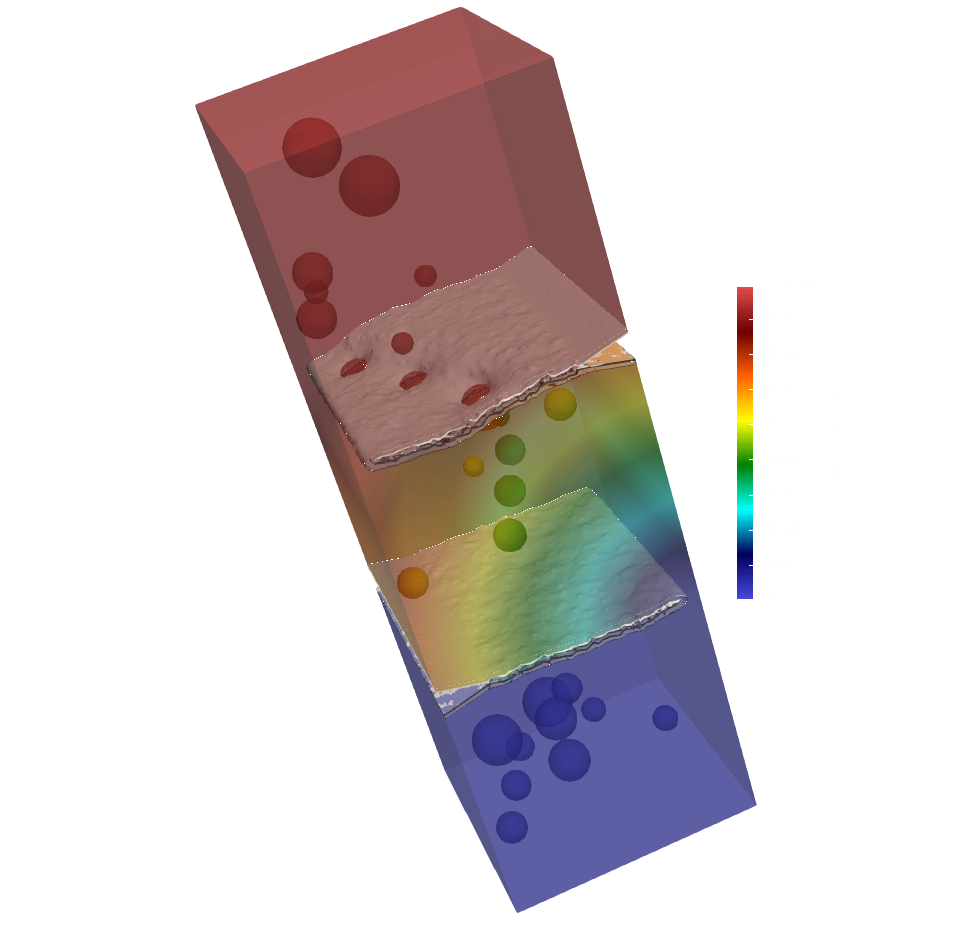
\includegraphics[width=0.45\textwidth]{./Images/rainbow-test1.png}
    \caption{Perforated concrete bar cracking.}
    \label{fig:rainbow}
\end{figure}

\begin{figure}
	\centering
	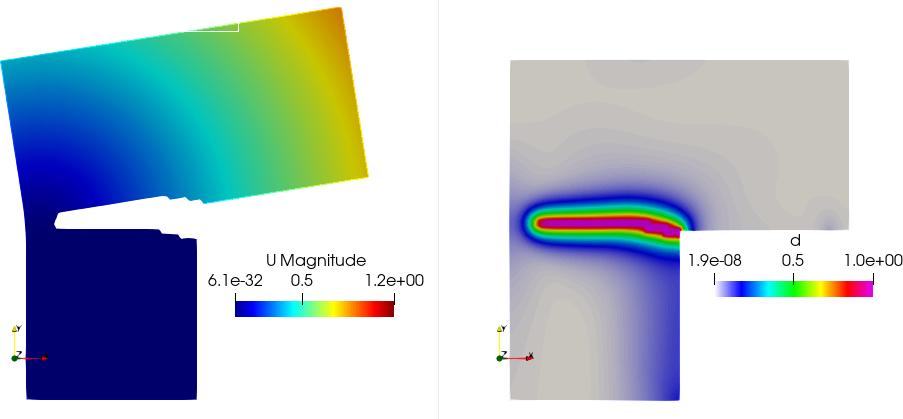
\includegraphics[width=0.6\textwidth]{./Images/fract-1.png}
	\caption{Point loading causing fracture in L-shaped material.}
	\label{fig:fract-1}
\end{figure}

\begin{figure}
    \centering
    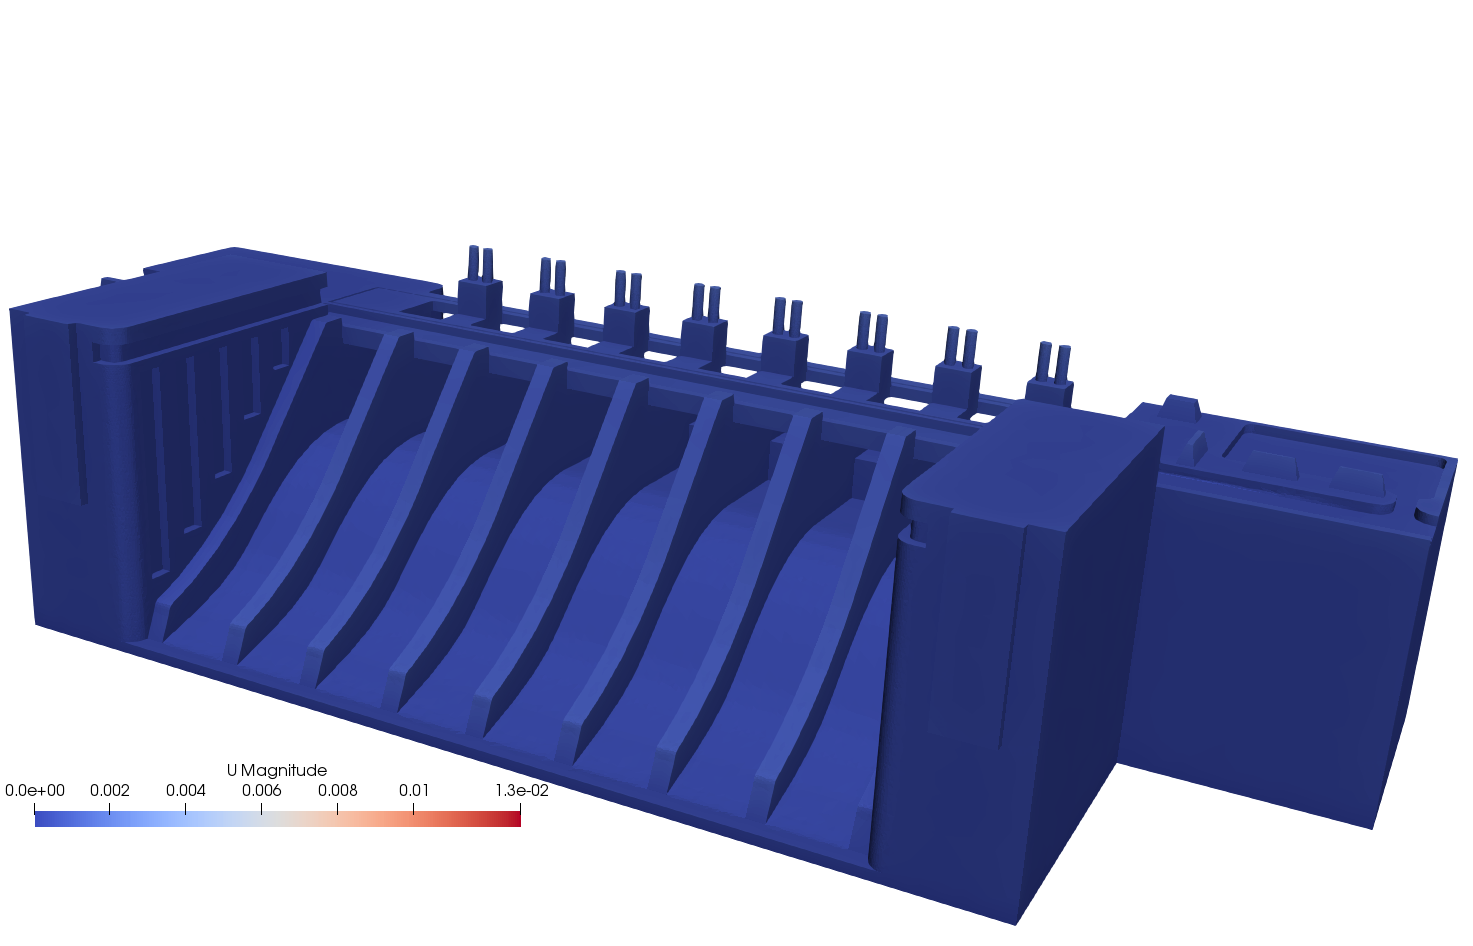
\includegraphics[width=0.45\textwidth]{./Images/dam1.png}    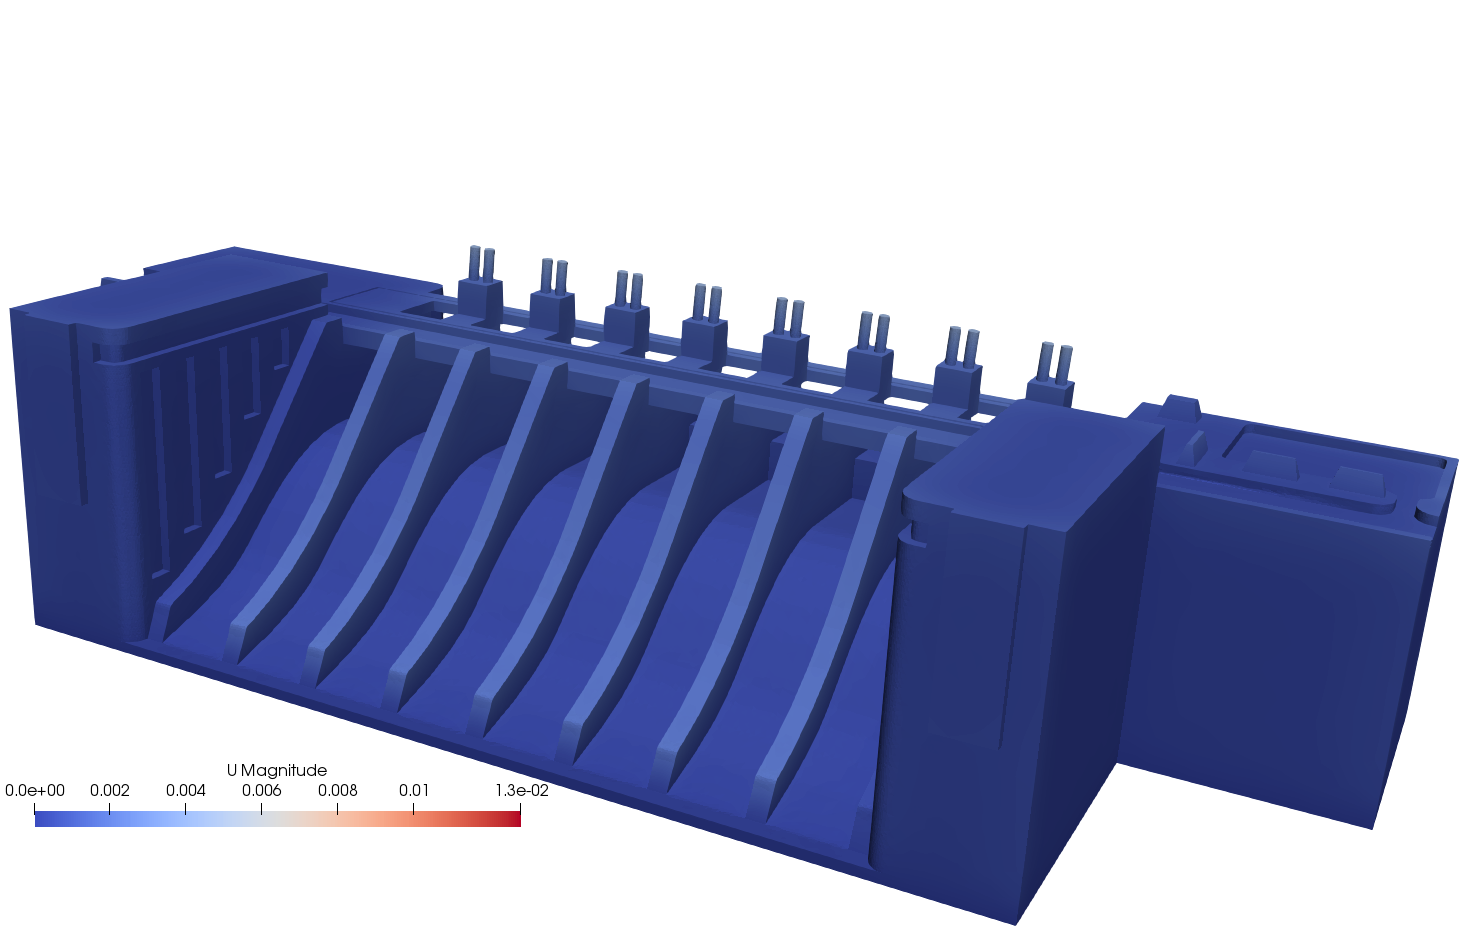
\includegraphics[width=0.45\textwidth]{./Images/dam2.png}\\
    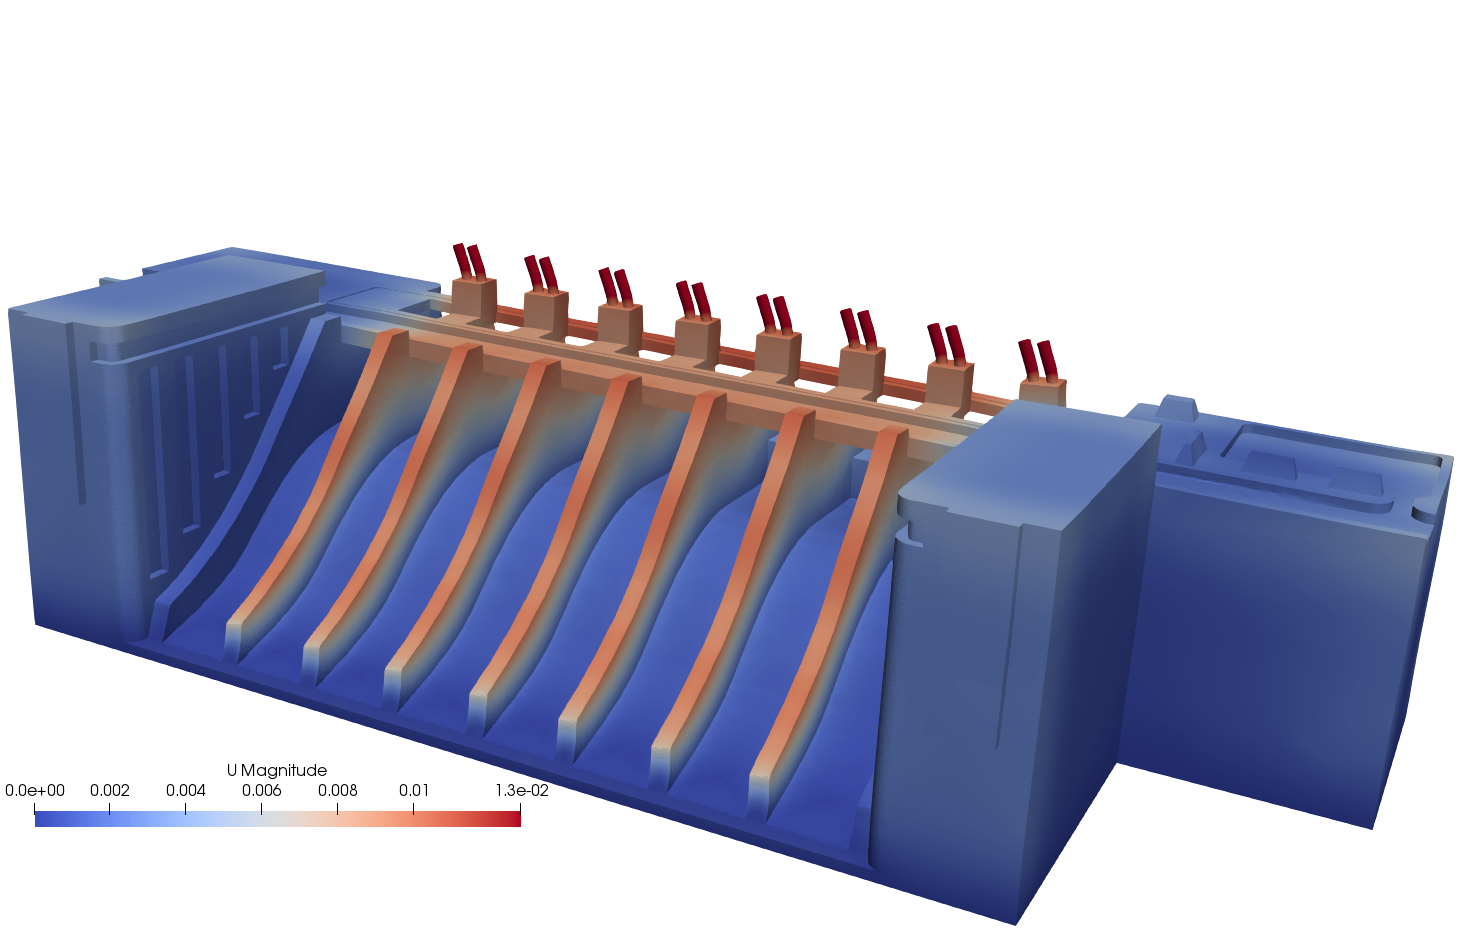
\includegraphics[width=0.45\textwidth]{./Images/dam3.png}
    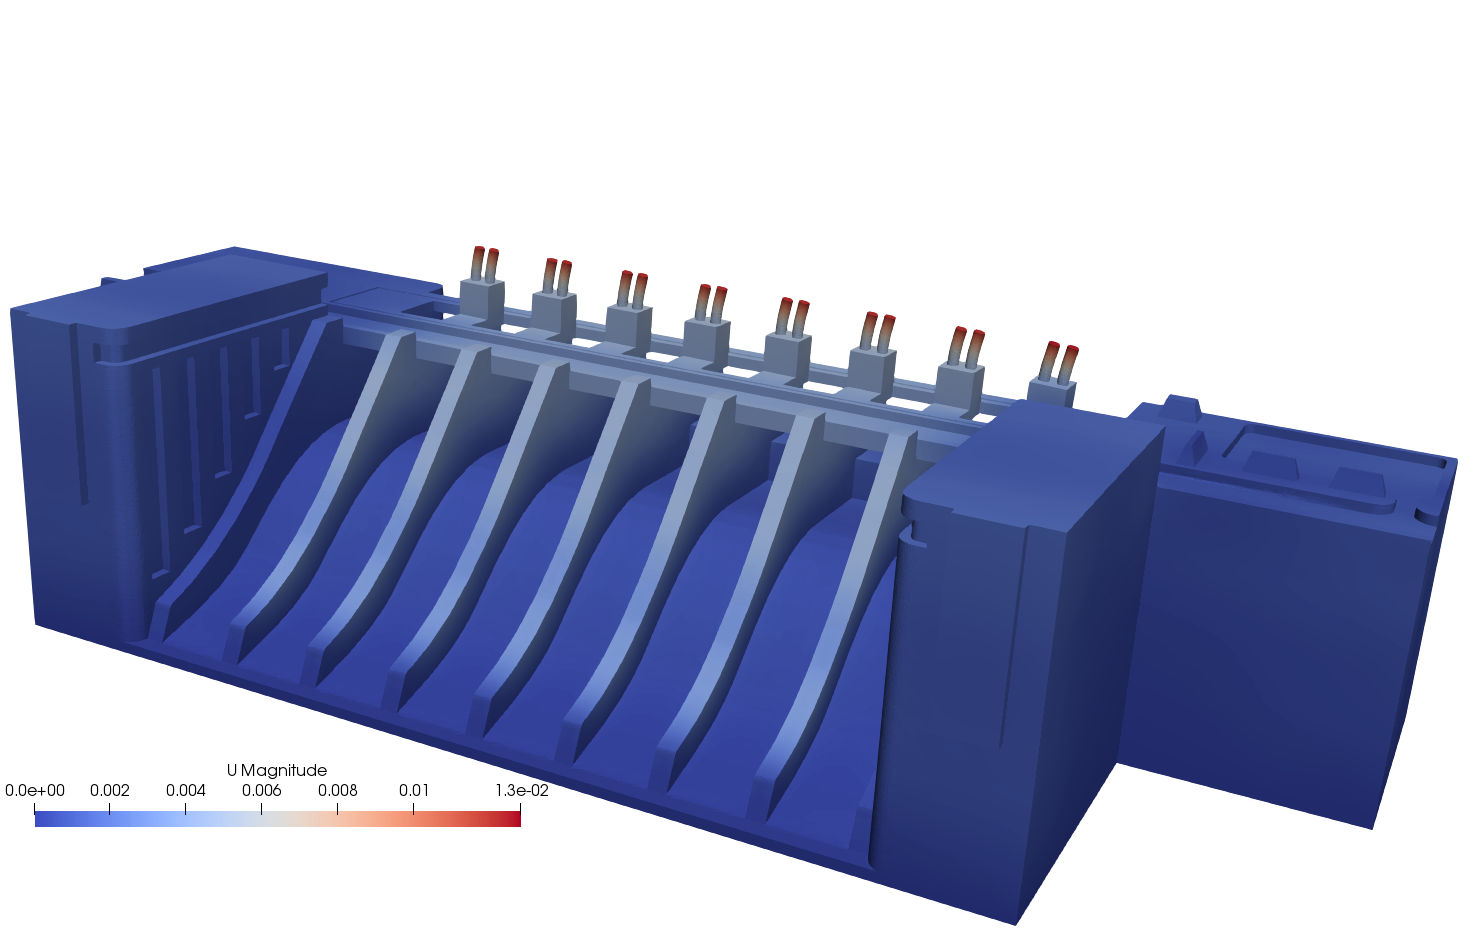
\includegraphics[width=0.45\textwidth]{./Images/dam4.png}
    \caption{Full scale dam under seismic load.}
    \label{fig:dam}
\end{figure}

\begin{figure}
    \centering
    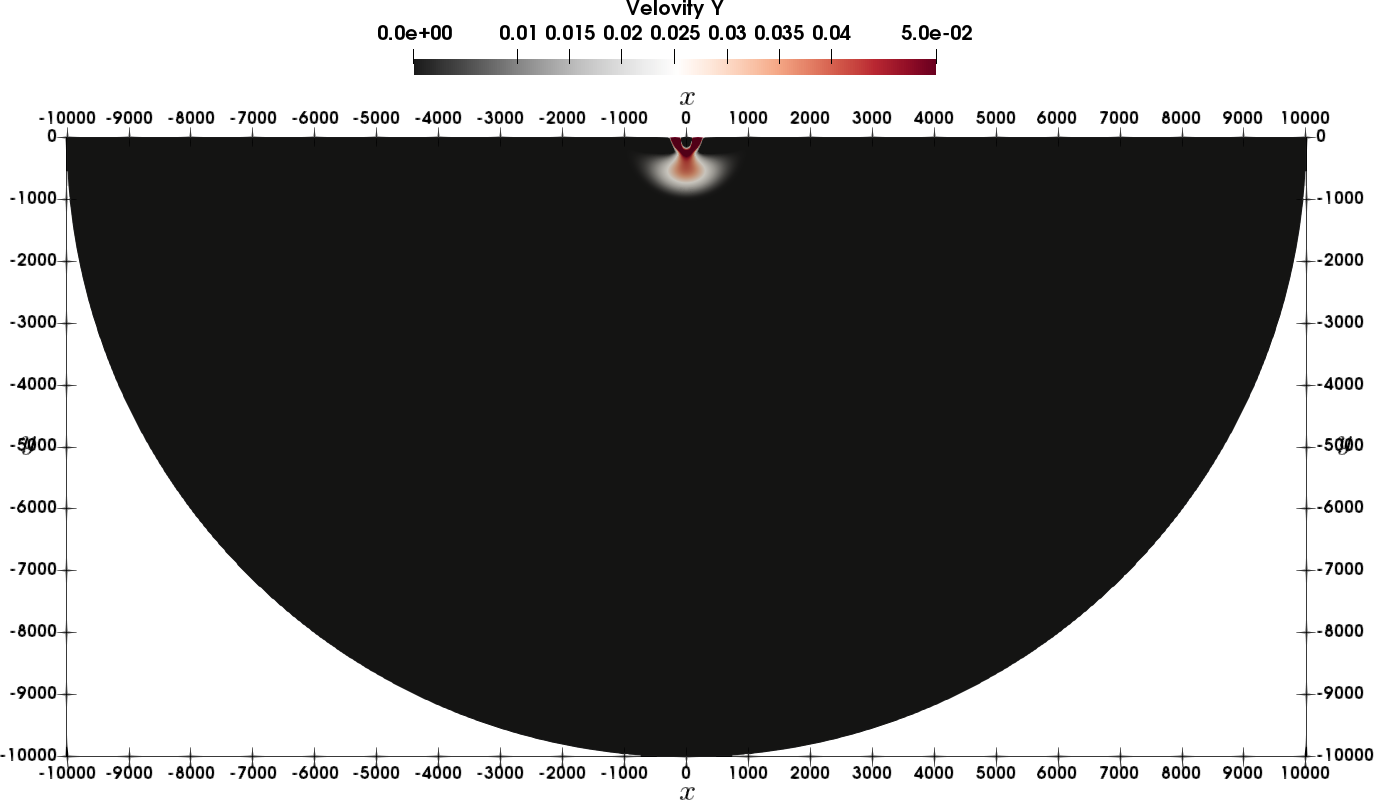
\includegraphics[width=0.3\textwidth]{./Images/t1-large.png}        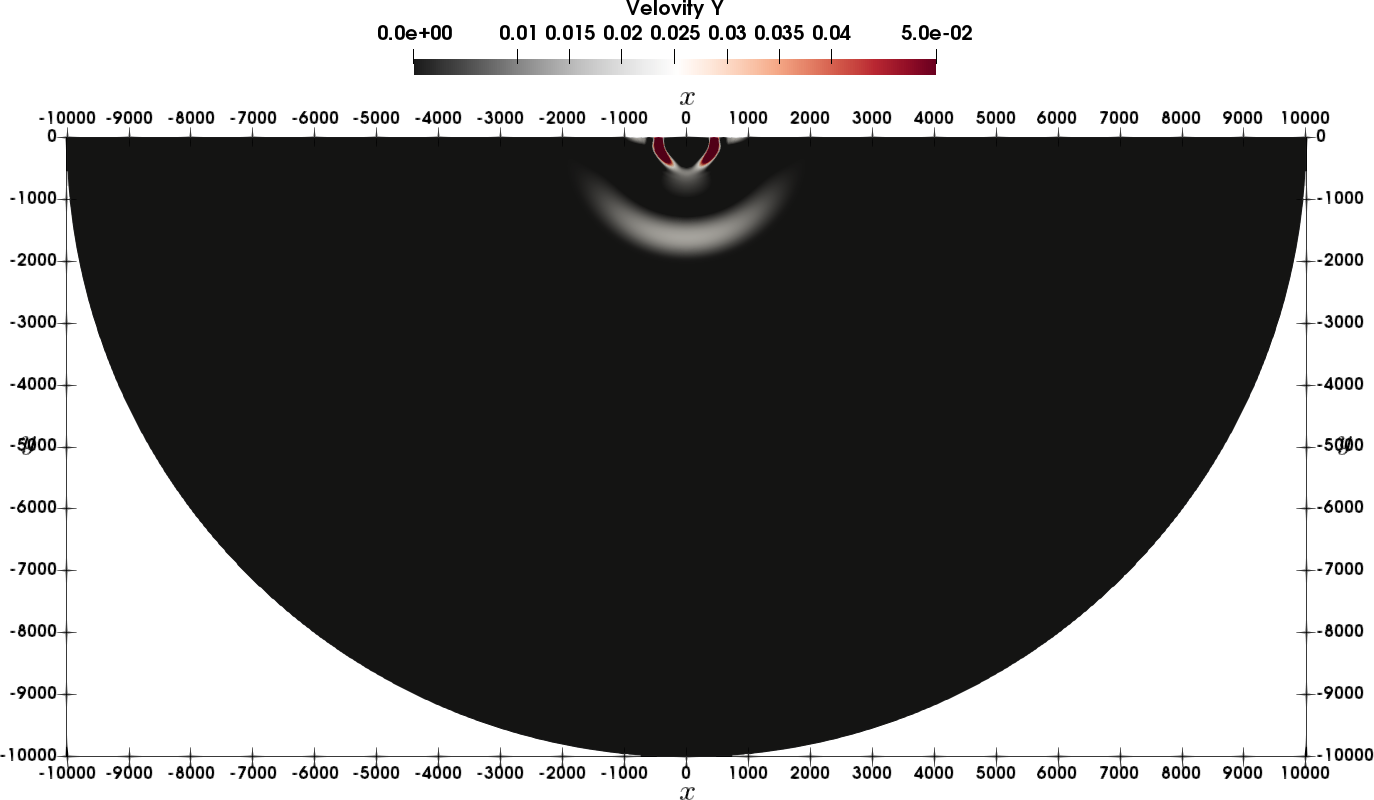
\includegraphics[width=0.3\textwidth]{./Images/t2-large.png}    
    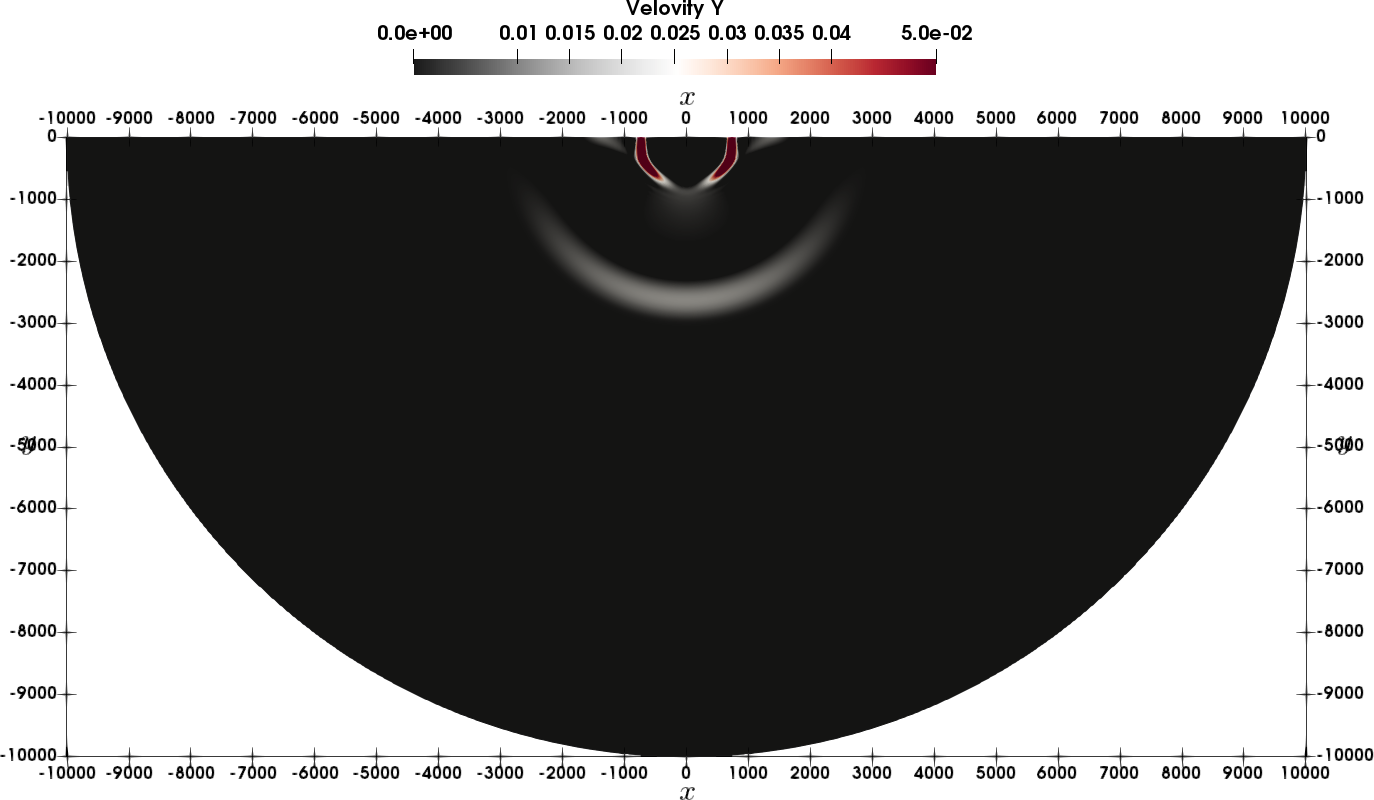
\includegraphics[width=0.3\textwidth]{./Images/t3-large.png}\\
    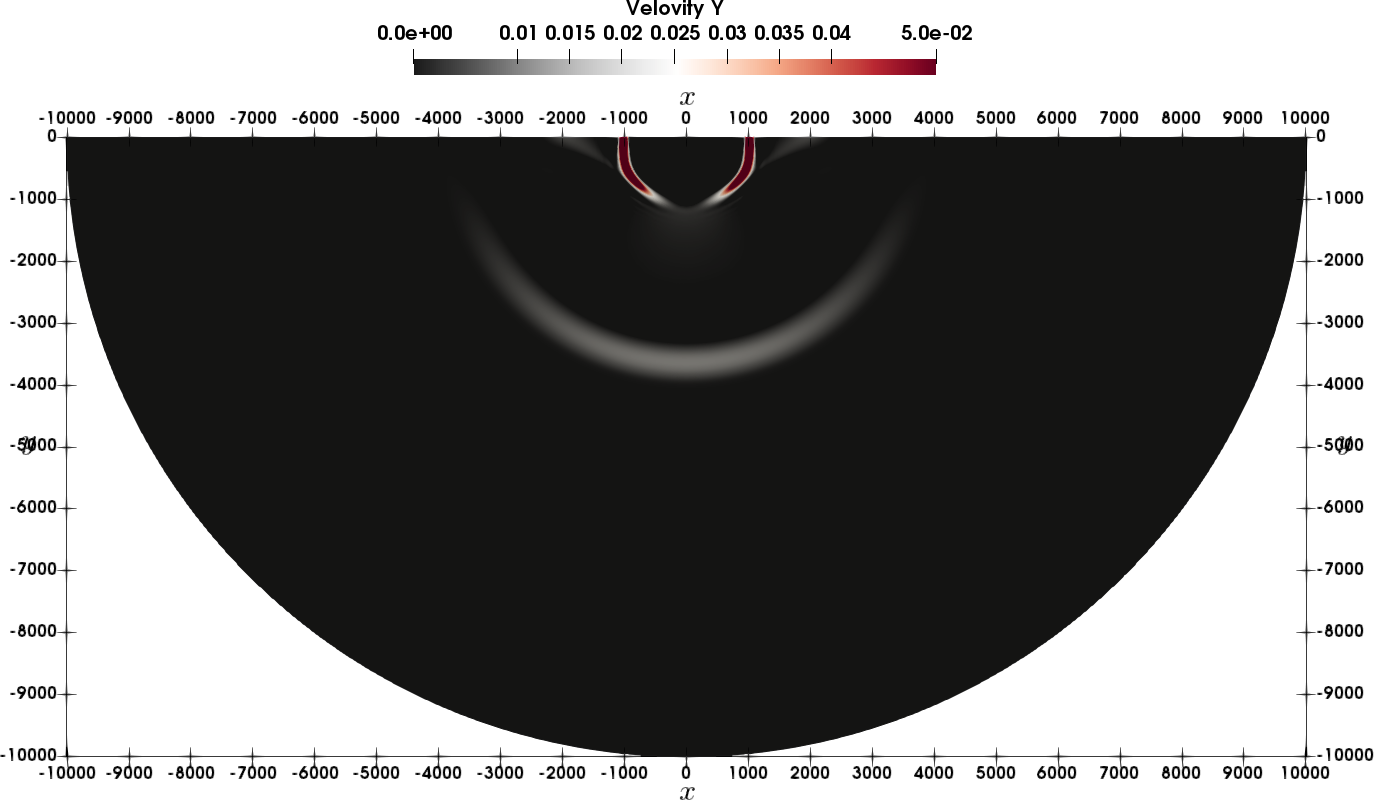
\includegraphics[width=0.3\textwidth]{./Images/t5-large.png}        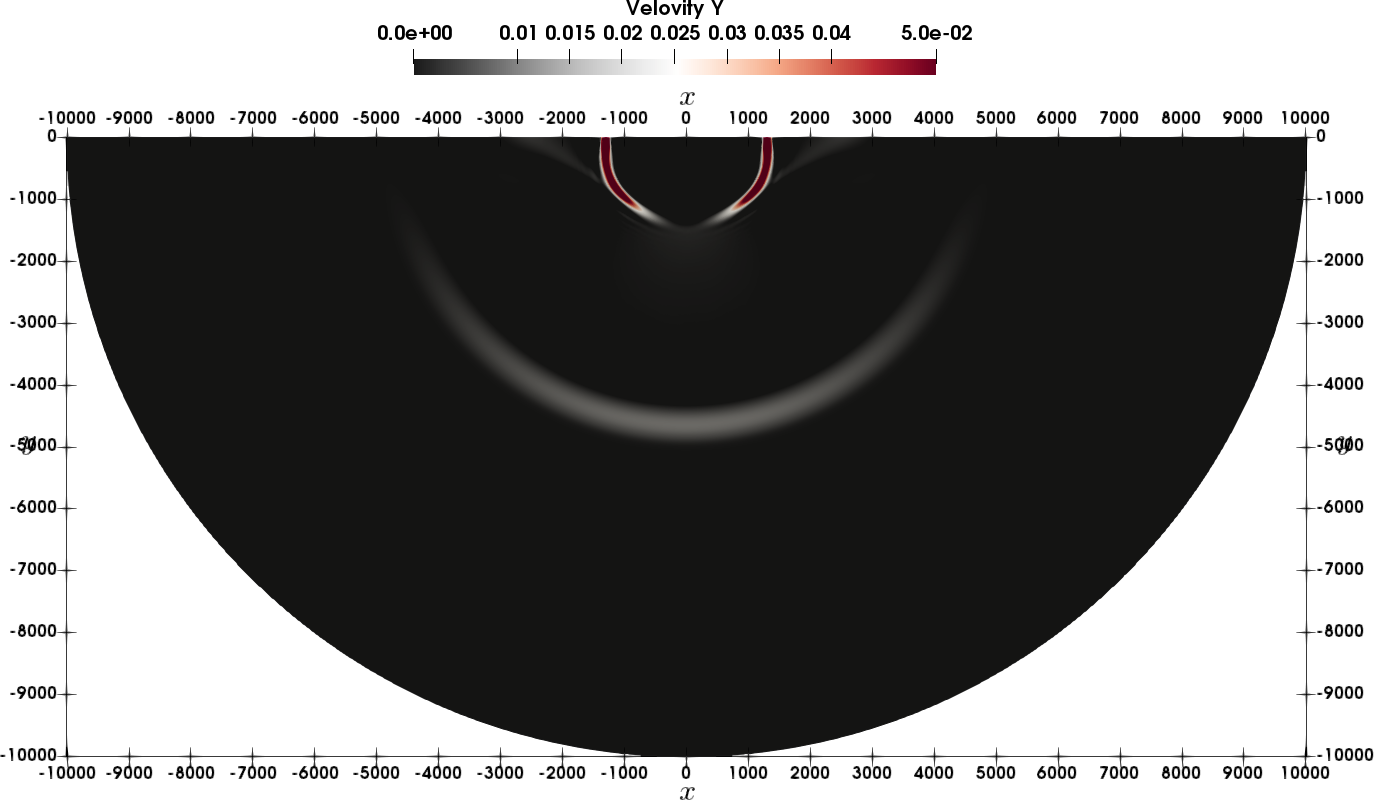
\includegraphics[width=0.3\textwidth]{./Images/t6-large.png}    
    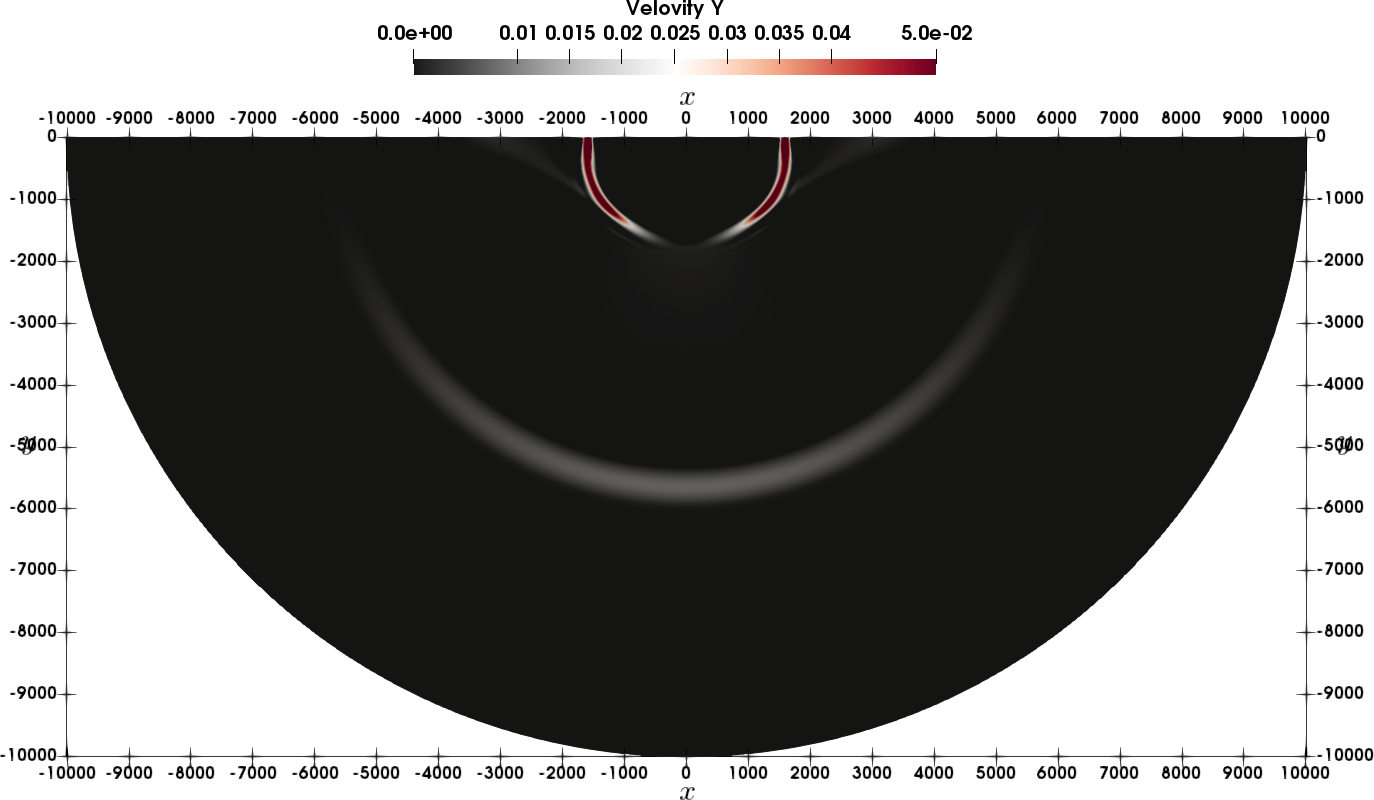
\includegraphics[width=0.3\textwidth]{./Images/t7-large.png}\\
    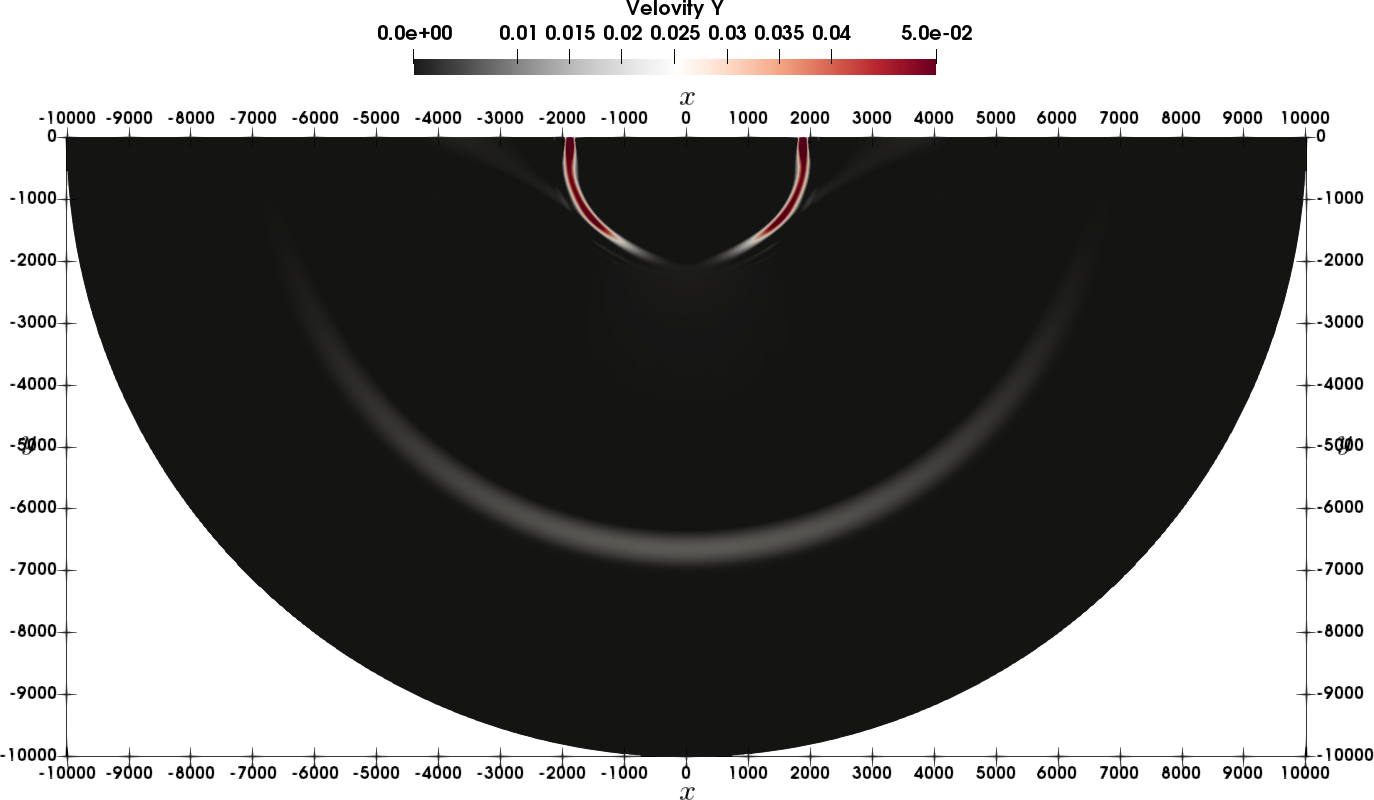
\includegraphics[width=0.3\textwidth]{./Images/t8-large.png}        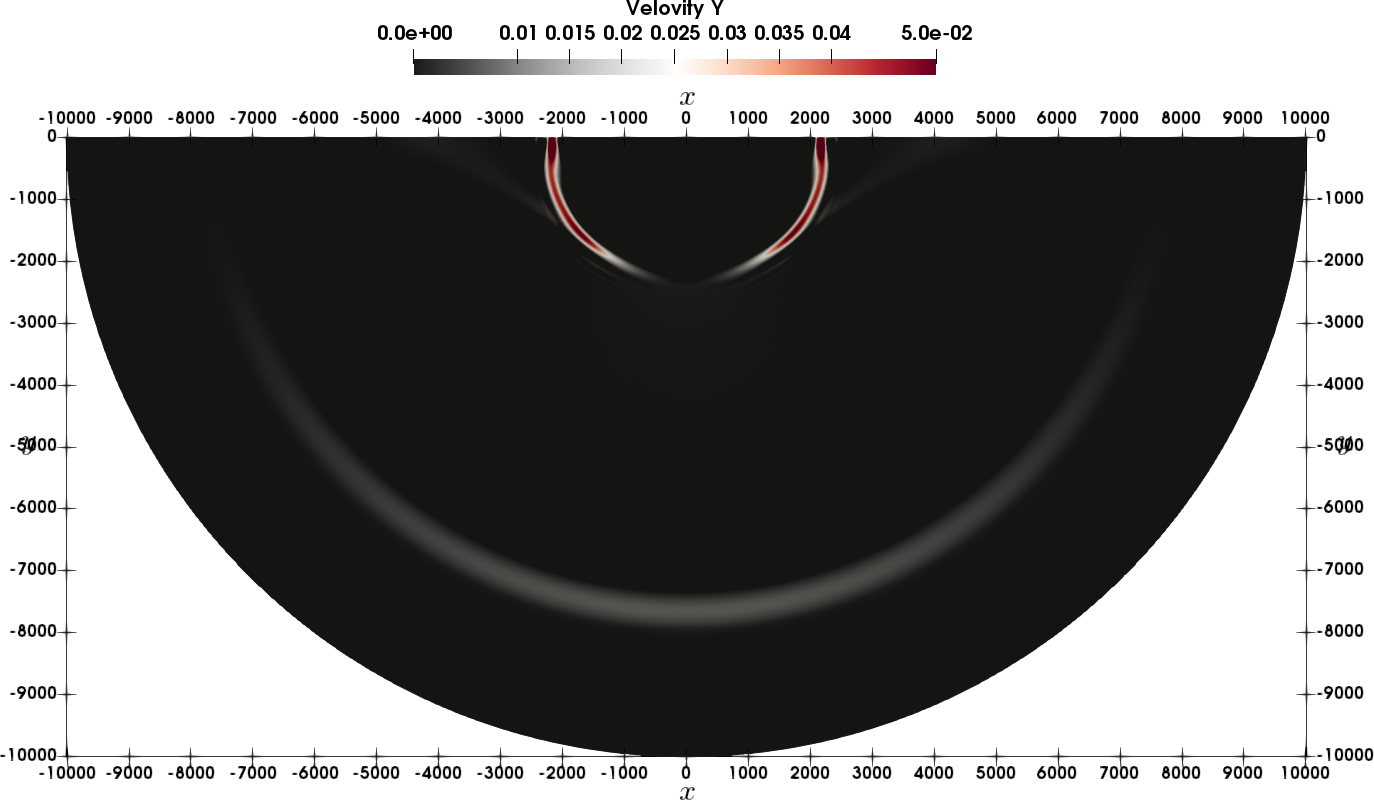
\includegraphics[width=0.3\textwidth]{./Images/t9-large.png}    
    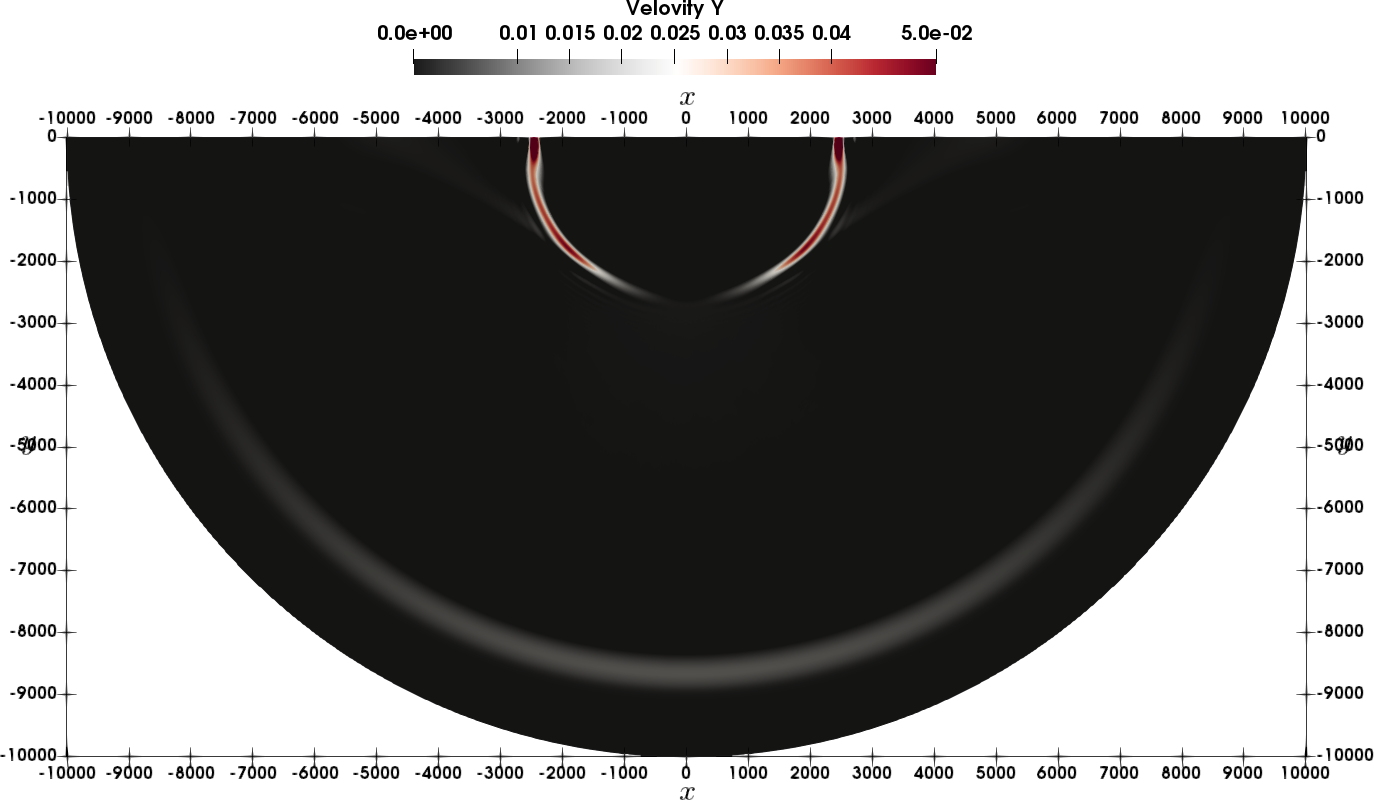
\includegraphics[width=0.3\textwidth]{./Images/t10-large.png}\\
    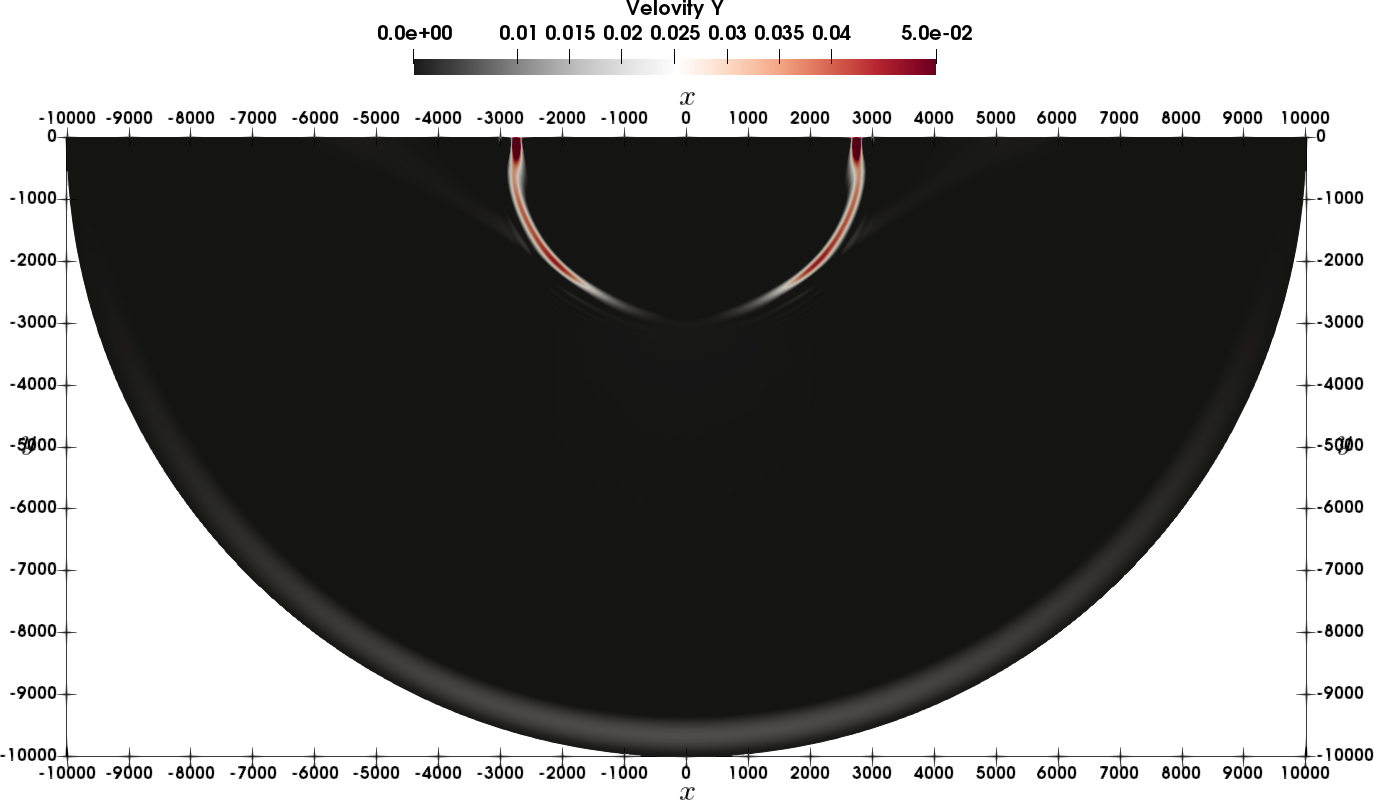
\includegraphics[width=0.3\textwidth]{./Images/t11-large.png}        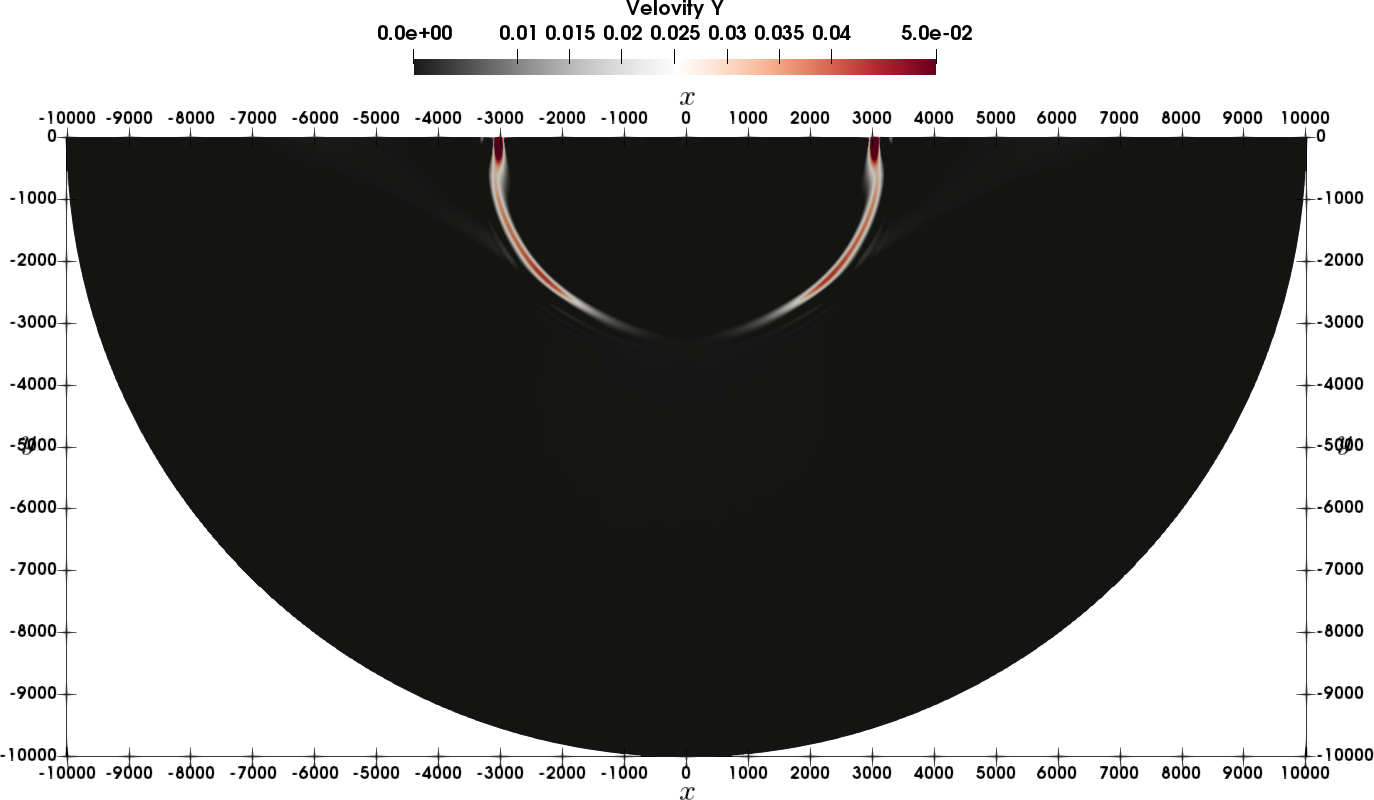
\includegraphics[width=0.3\textwidth]{./Images/t12-large.png}    
    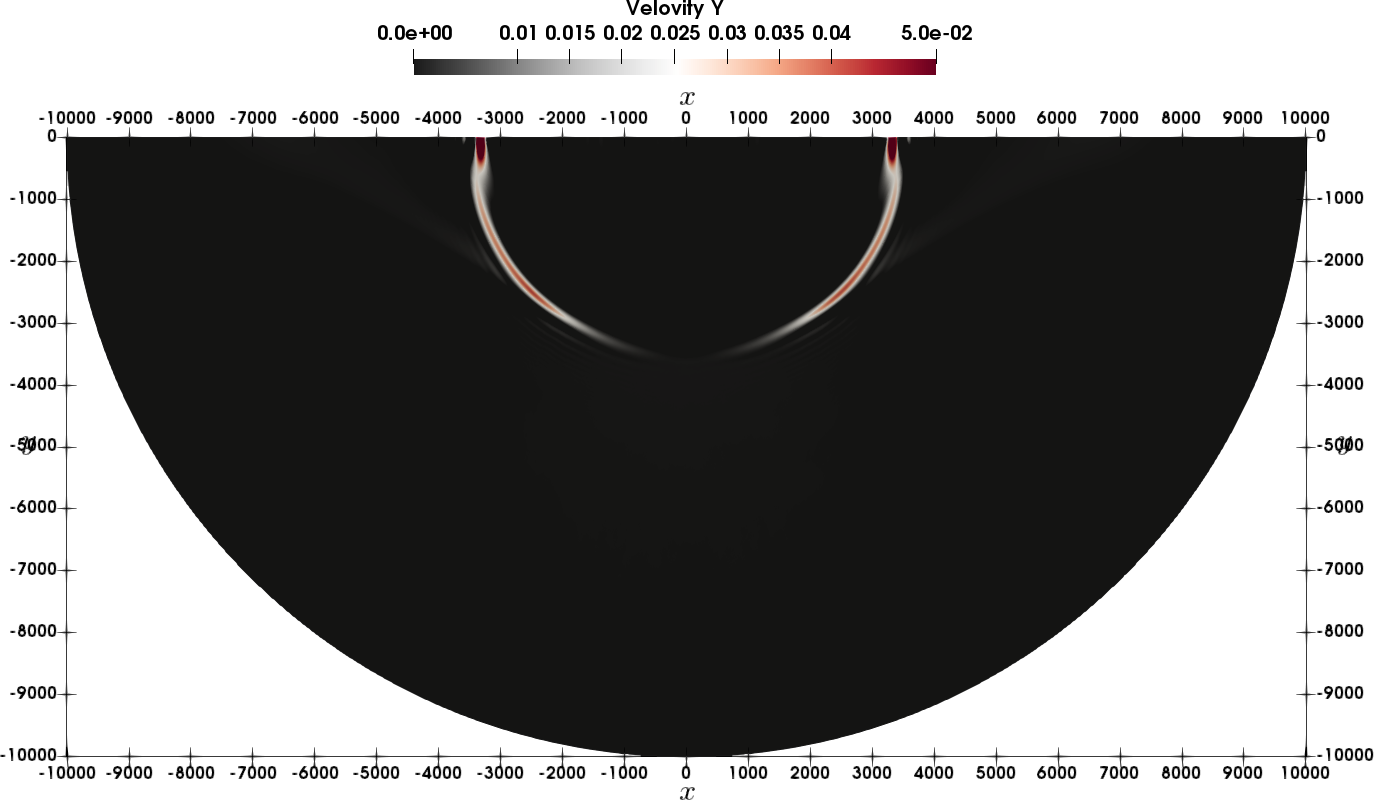
\includegraphics[width=0.3\textwidth]{./Images/t13-large.png}
    \caption{Seismic signal dispersion in soil.}
    \label{fig:soilsemi}
\end{figure}


\begin{figure}
    \centering
    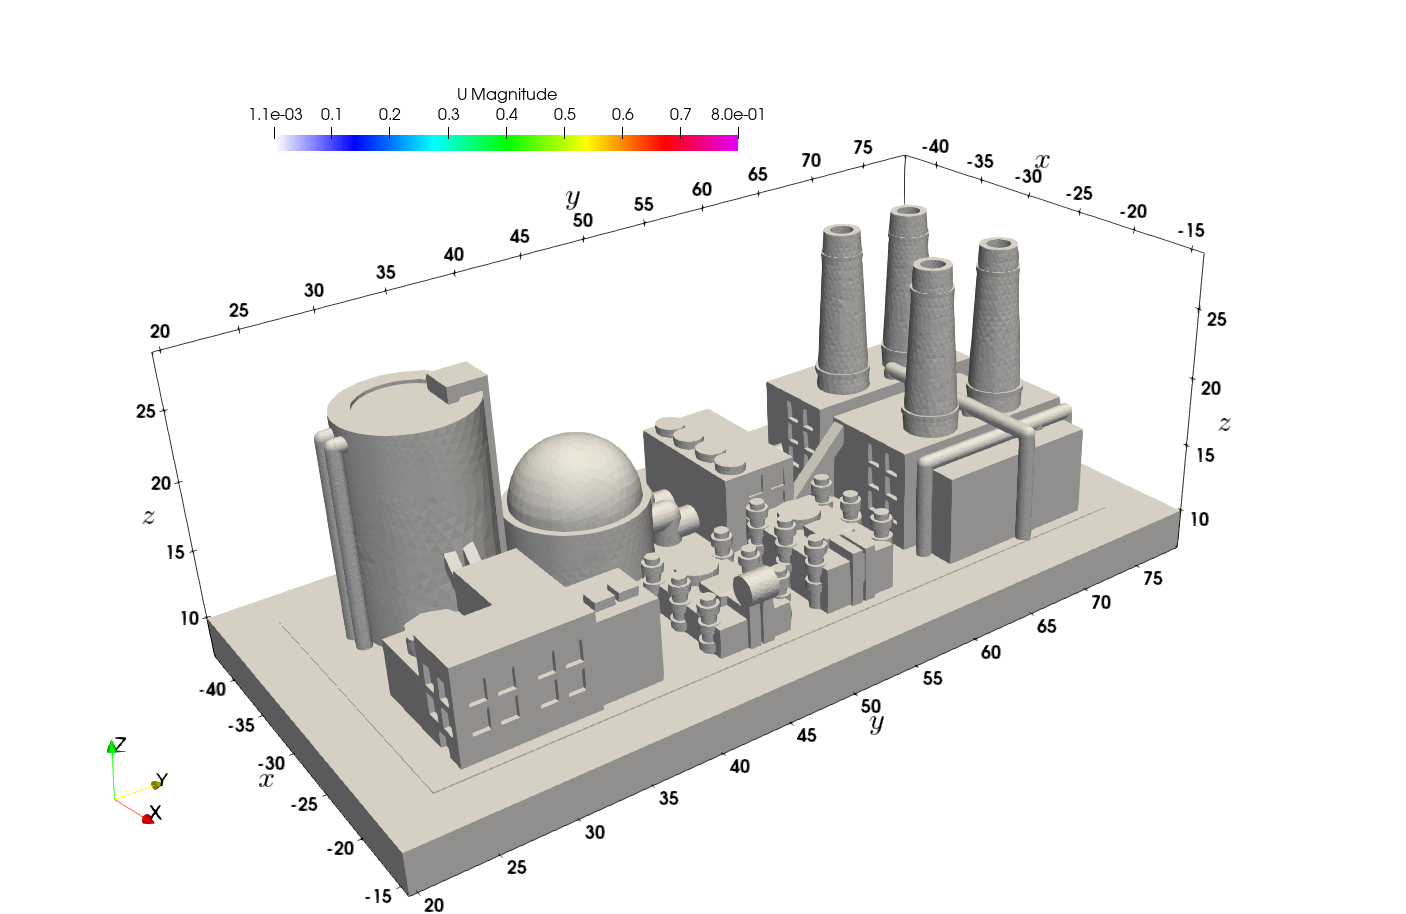
\includegraphics[width=0.65\textwidth]{./Images/t001.png}        
    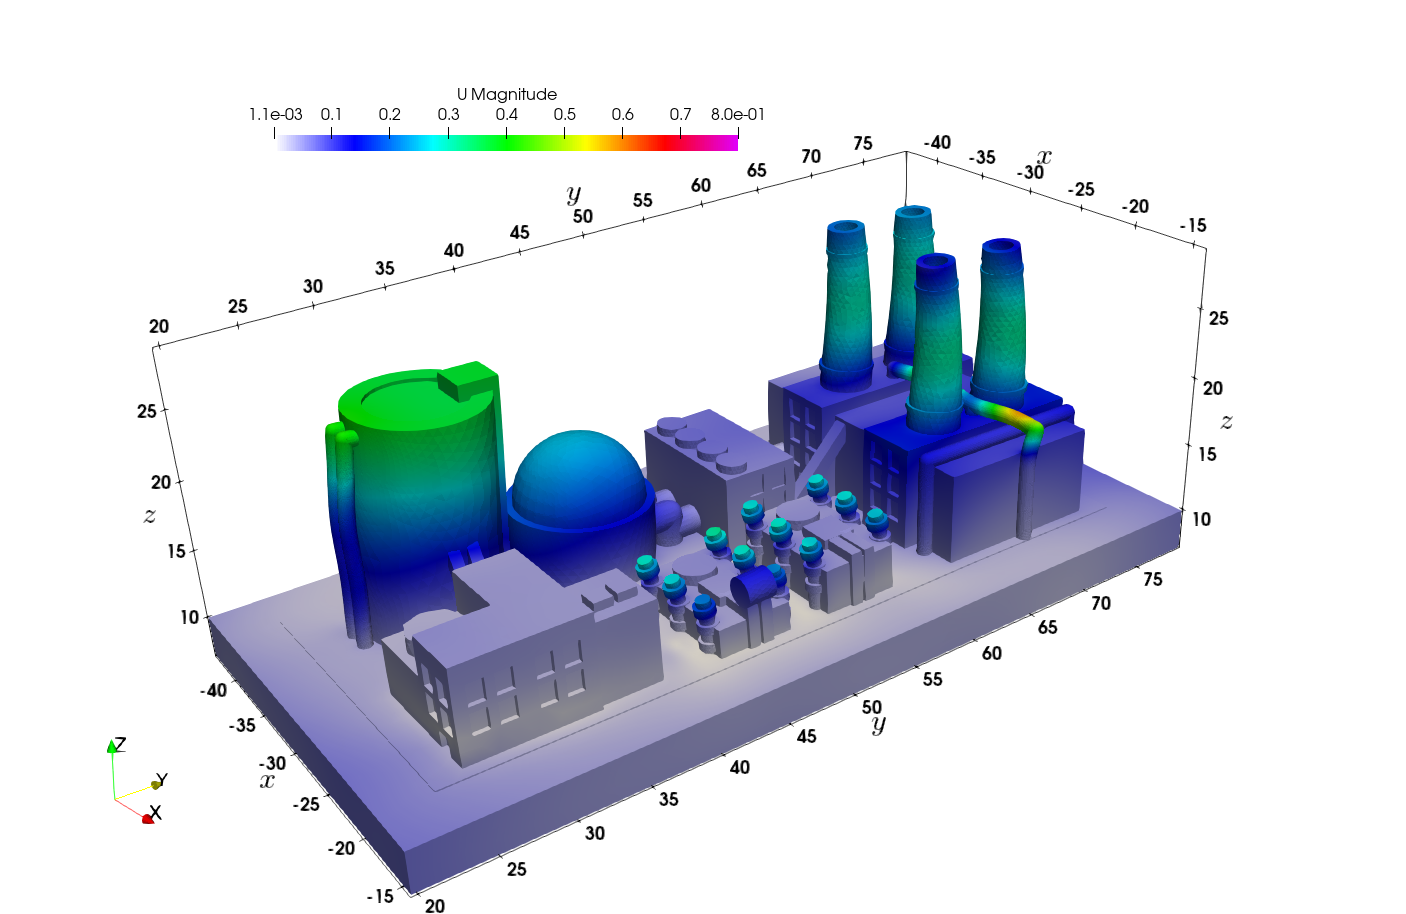
\includegraphics[width=0.65\textwidth]{./Images/t100.png}    
    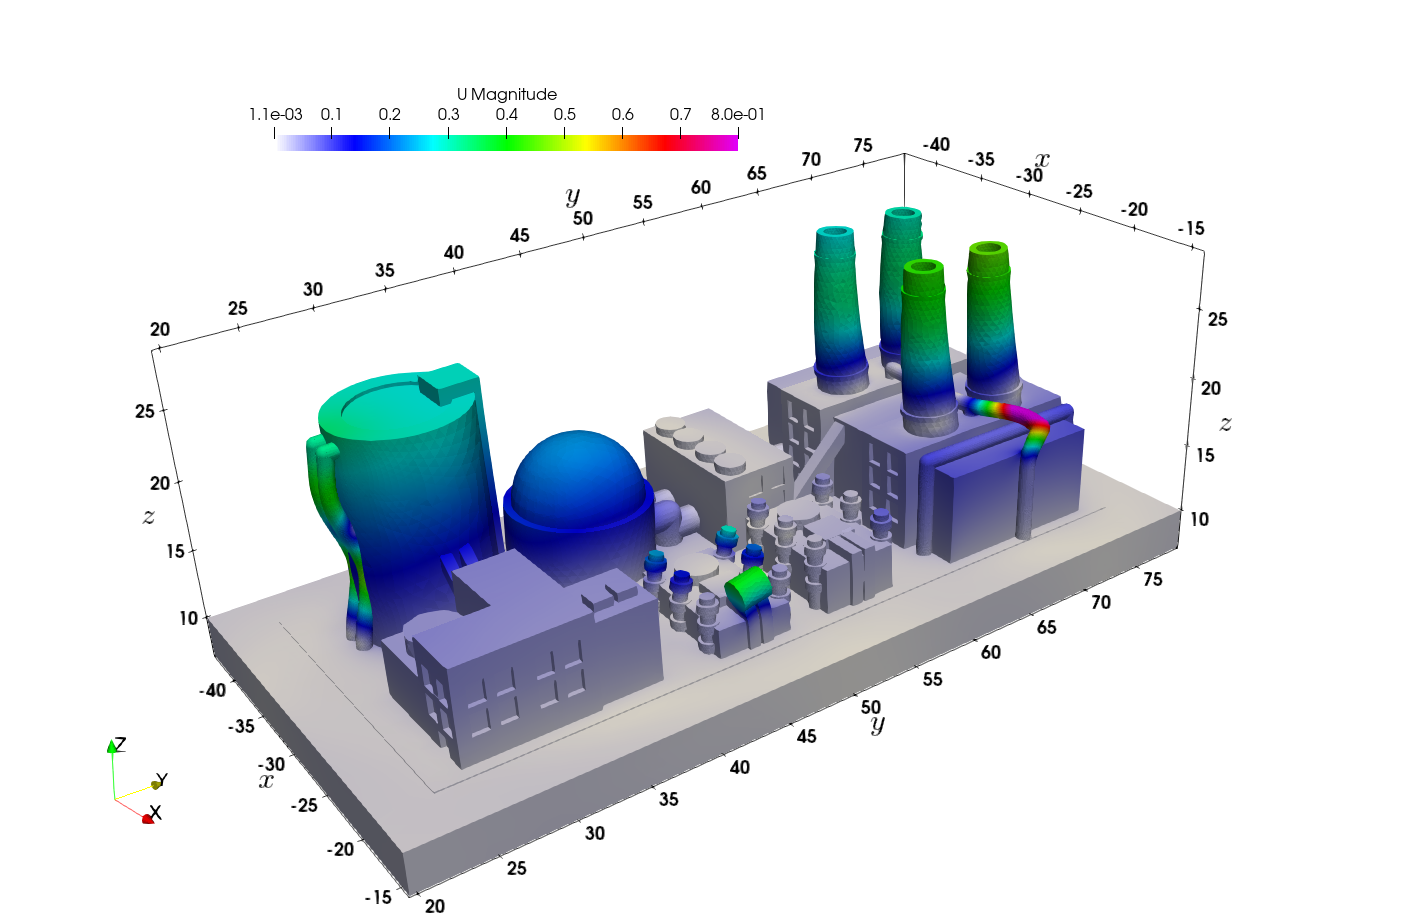
\includegraphics[width=0.65\textwidth]{./Images/t199.png} 
    \caption{Seismic signal on nuclear site.}
    \label{fig:nuclearplant}
\end{figure}

\begin{figure}
	\centering
	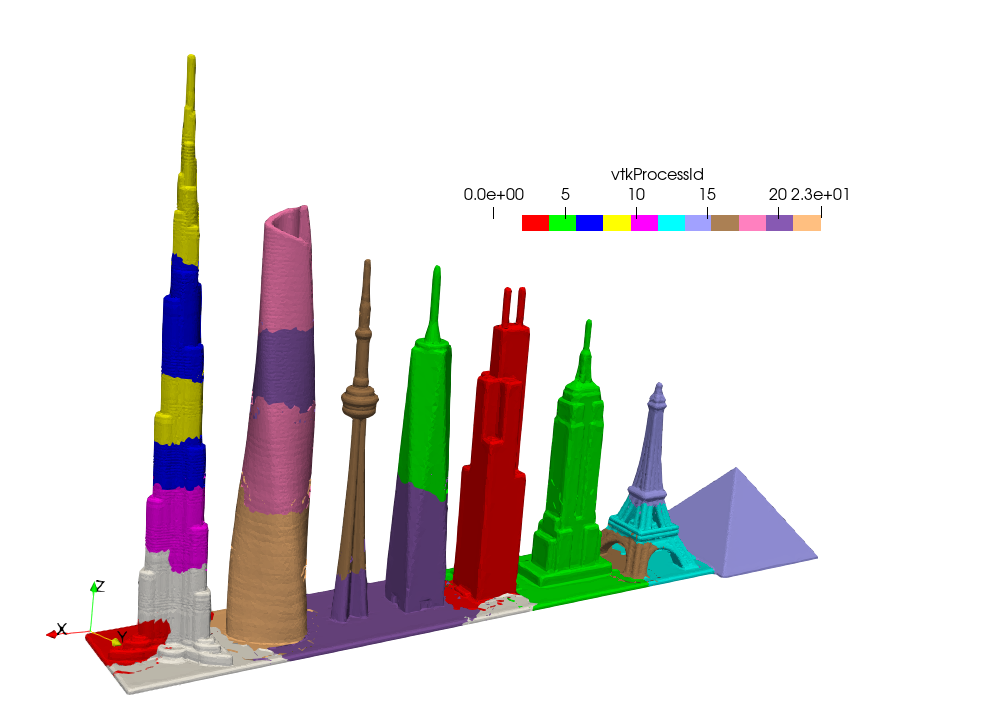
\includegraphics[width=0.65\textwidth]{./Images/partitioned.png}        
	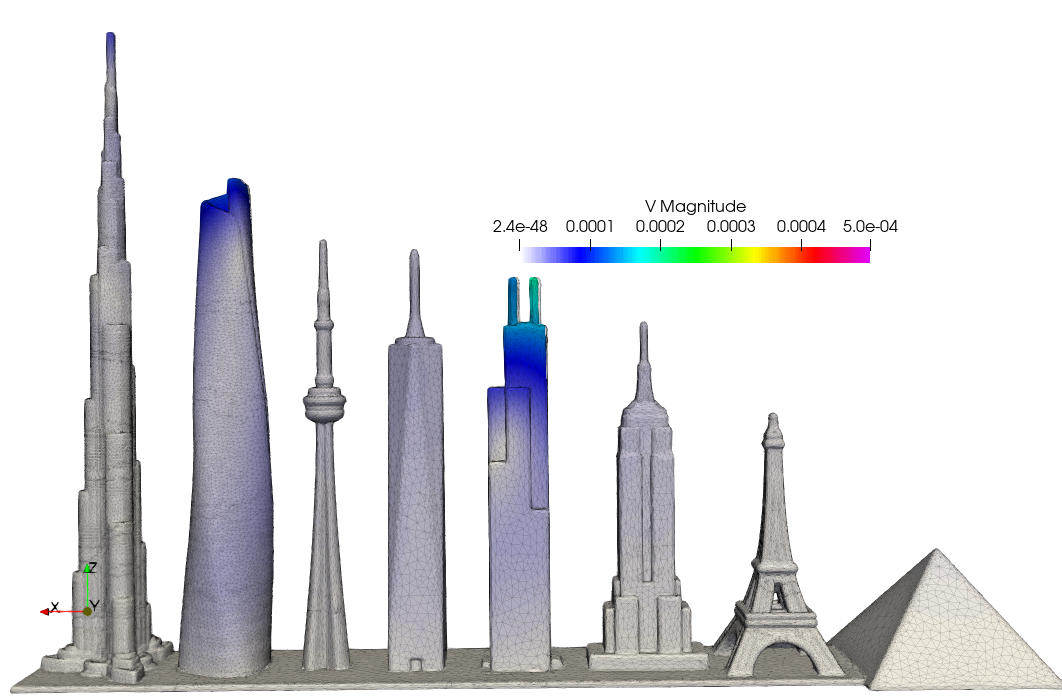
\includegraphics[width=0.65\textwidth]{./Images/frame0000.png}    
	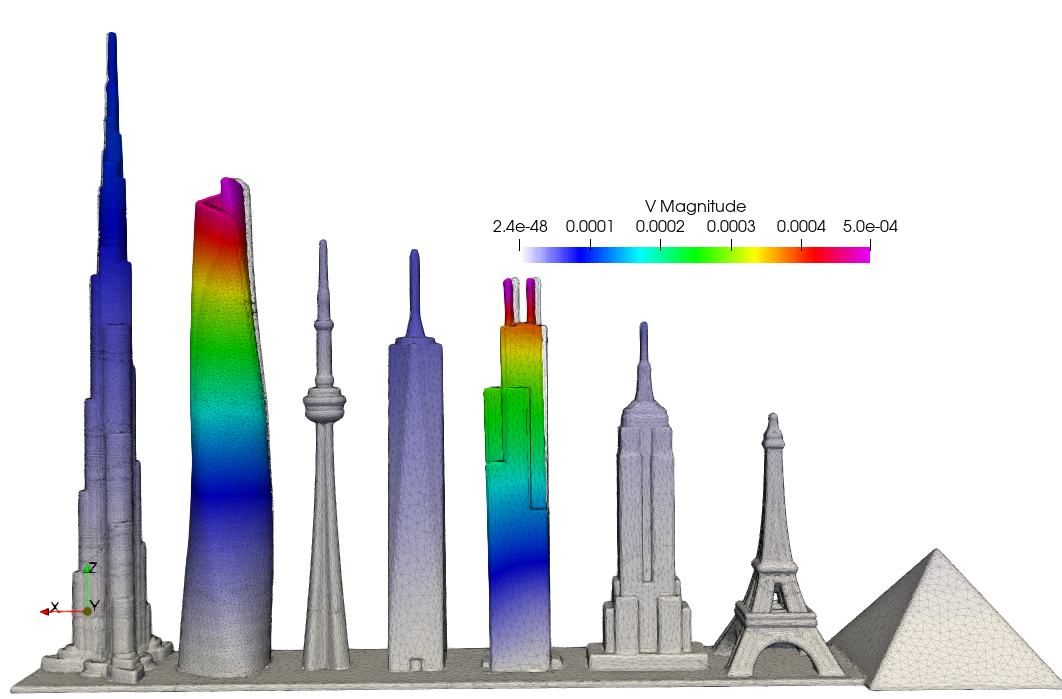
\includegraphics[width=0.65\textwidth]{./Images/frame0080.png} 
	\caption{Seismic signal on famous world buildings.}
	\label{fig:buildings}
\end{figure}


\begin{figure}
	\centering
	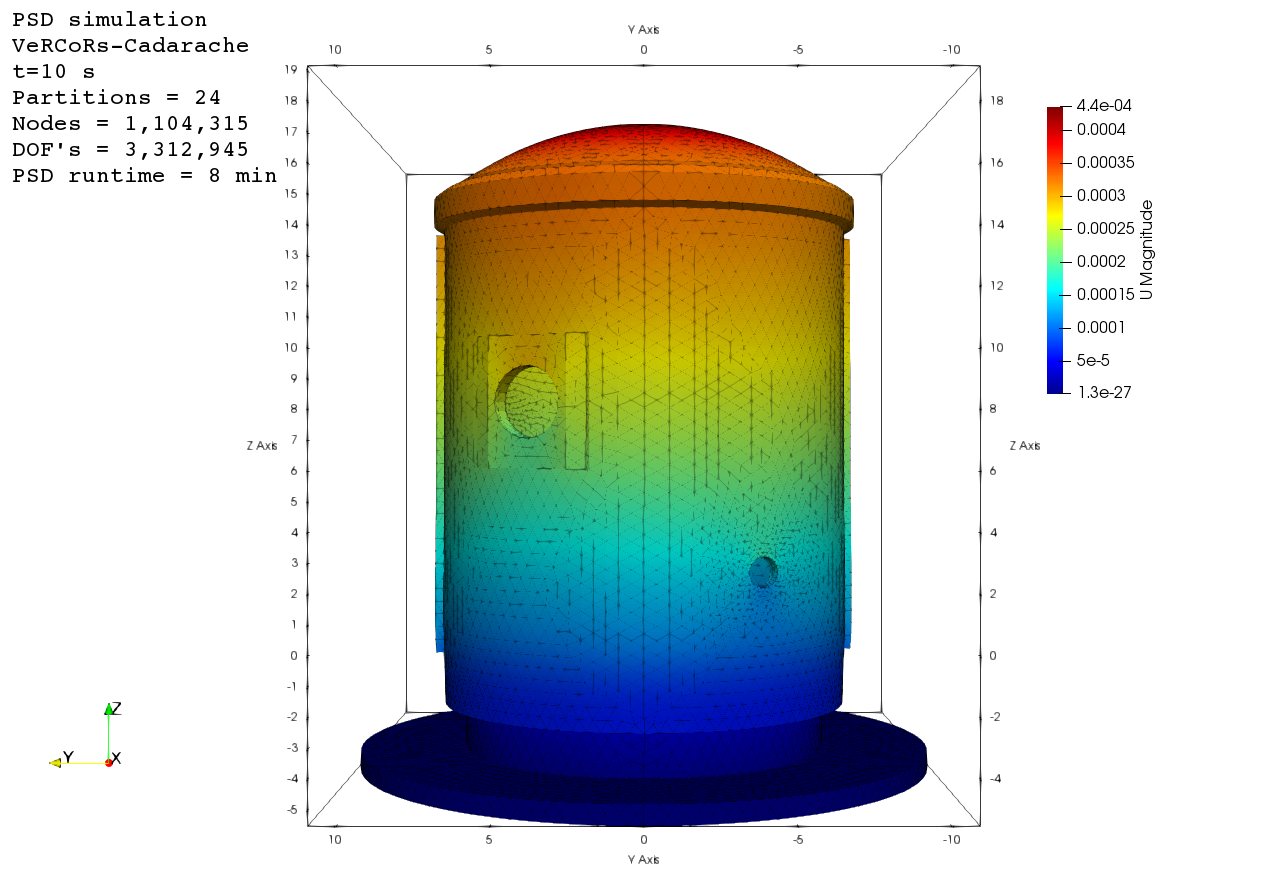
\includegraphics[width=0.45\textwidth]{./Images/vercor0000.png}        
	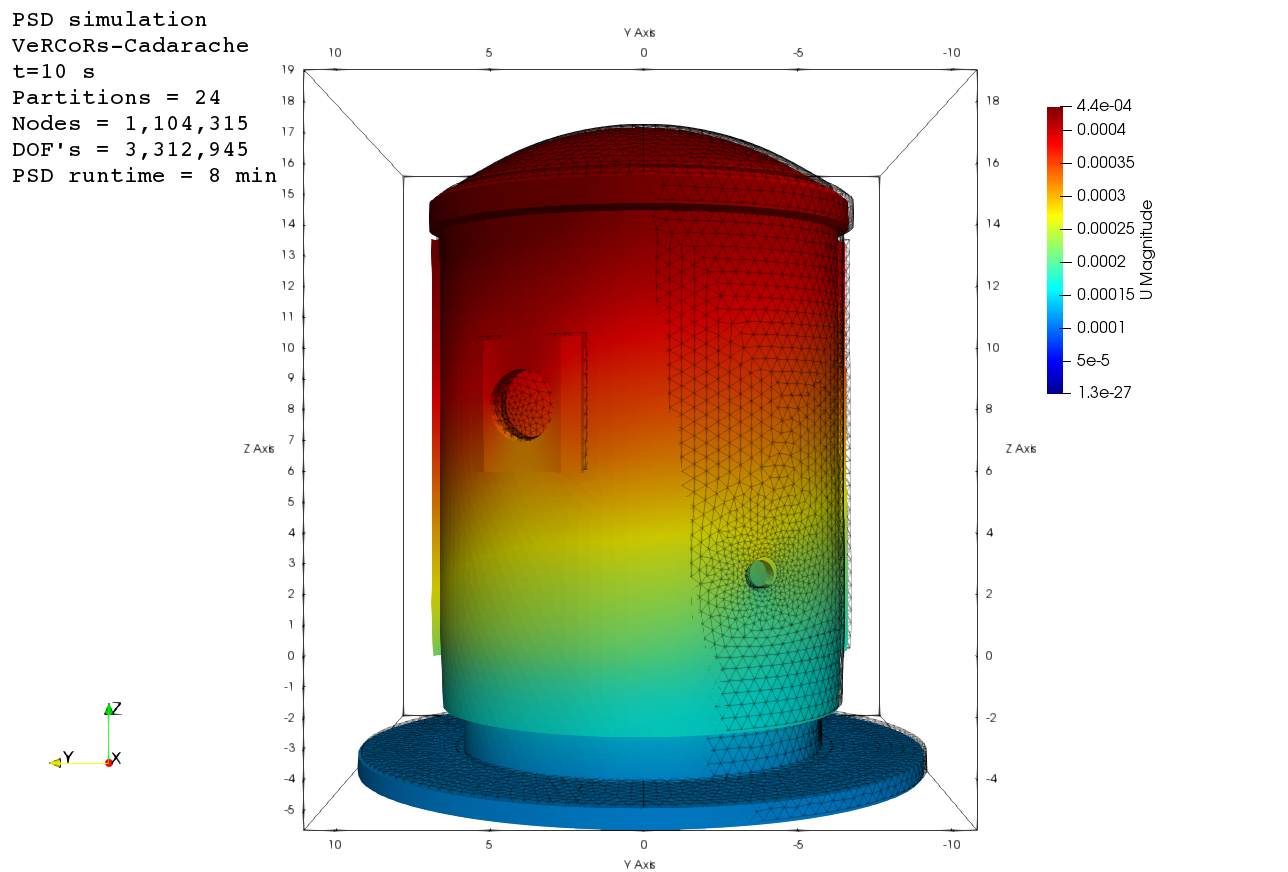
\includegraphics[width=0.45\textwidth]{./Images/vercor0111.png}\\    
	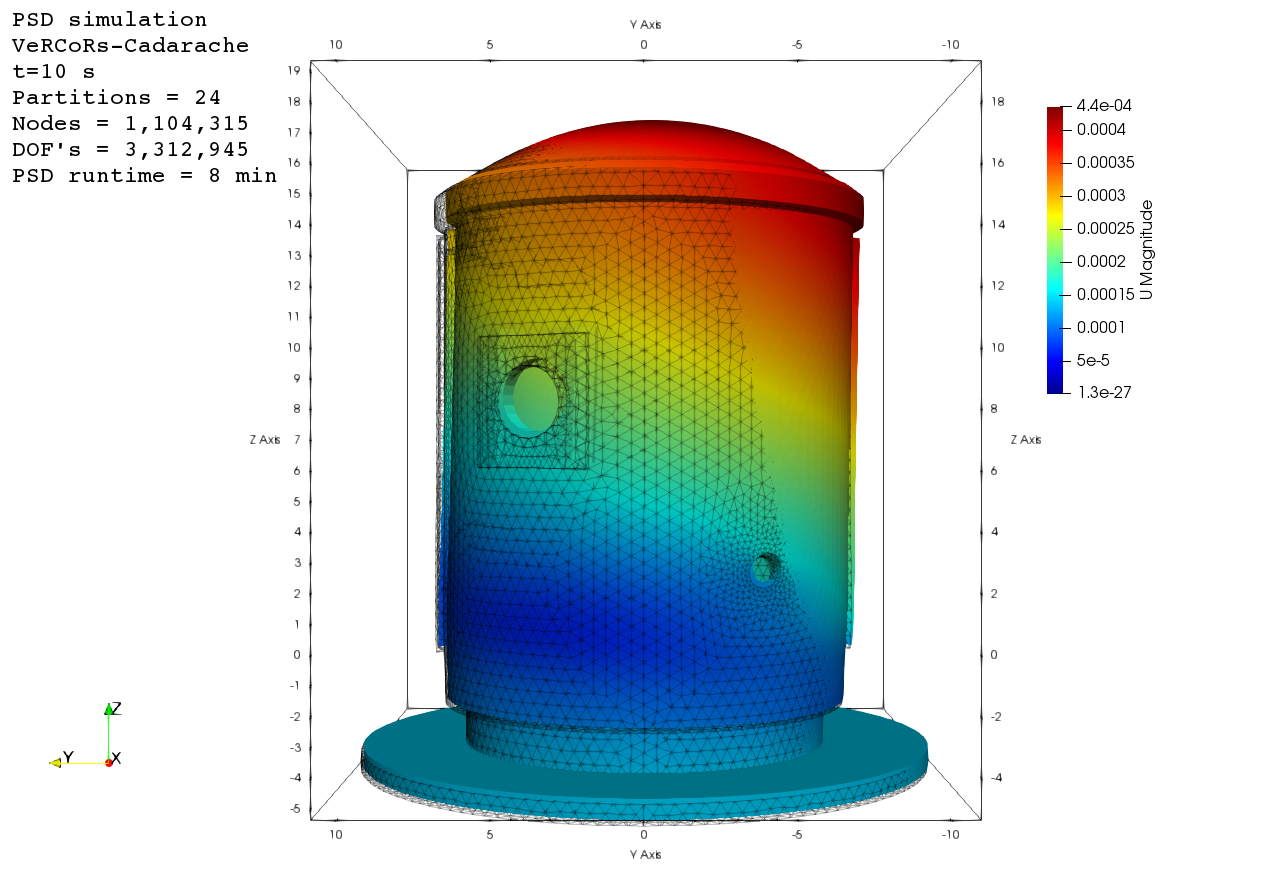
\includegraphics[width=0.45\textwidth]{./Images/vercor0119.png}
	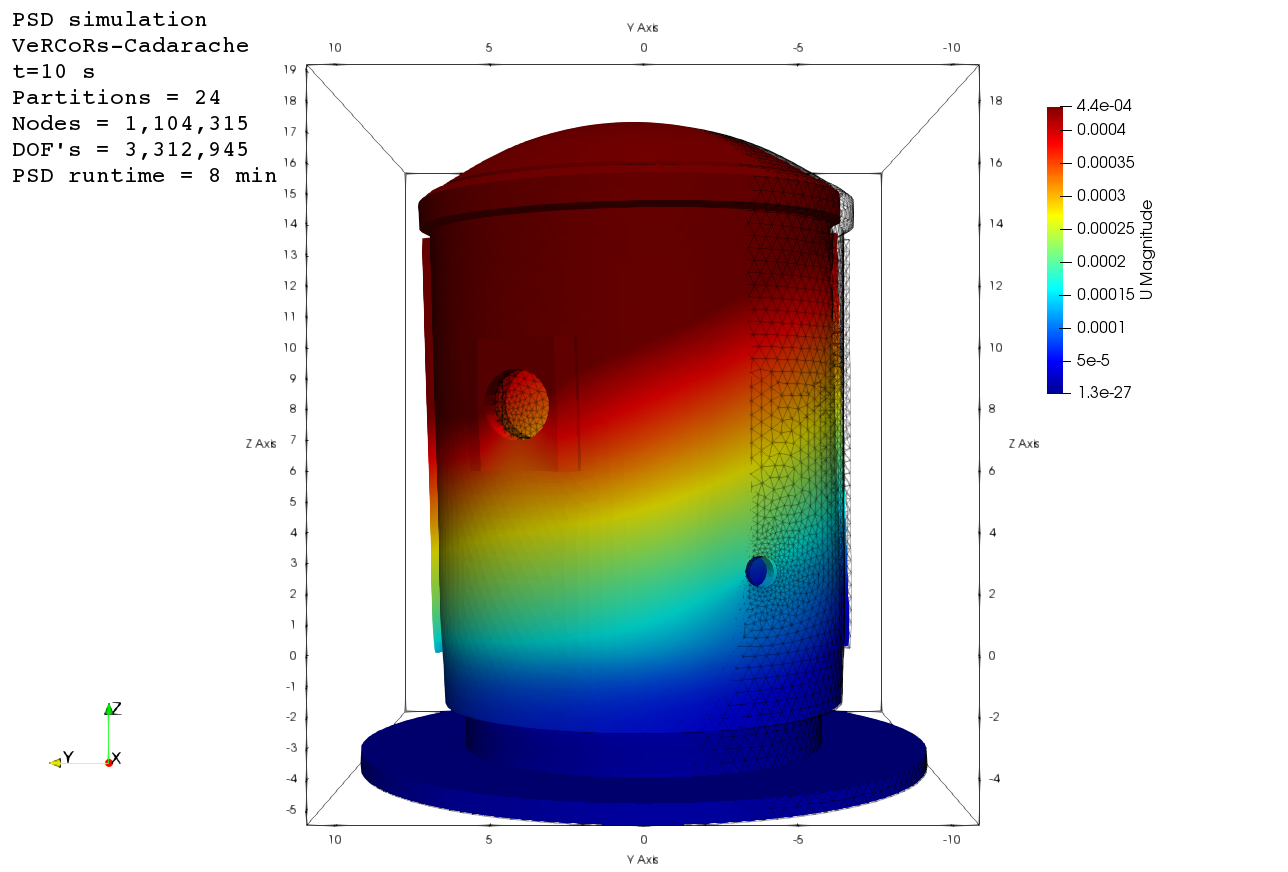
\includegraphics[width=0.45\textwidth]{./Images/vercor134.png}\\        
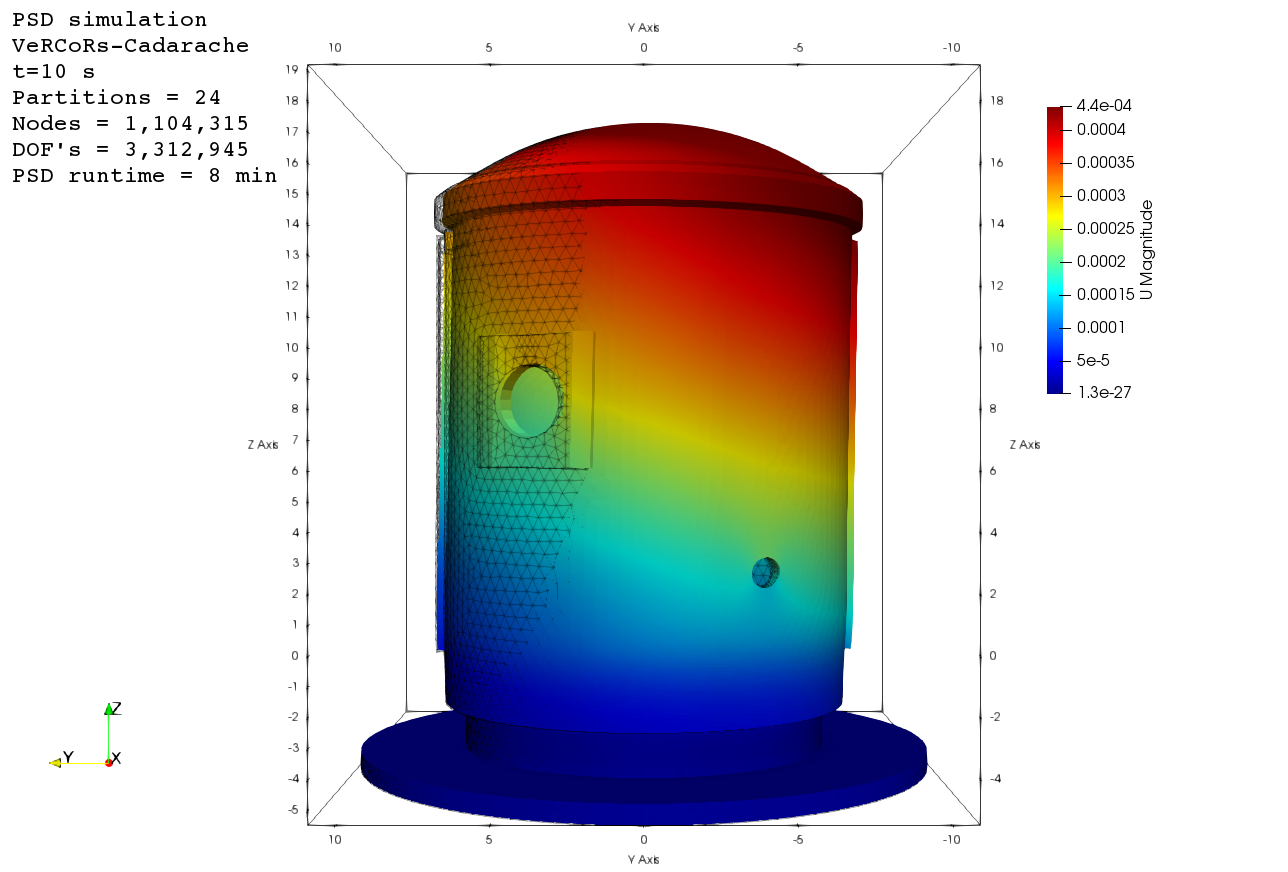
\includegraphics[width=0.45\textwidth]{./Images/vercor138.png}    
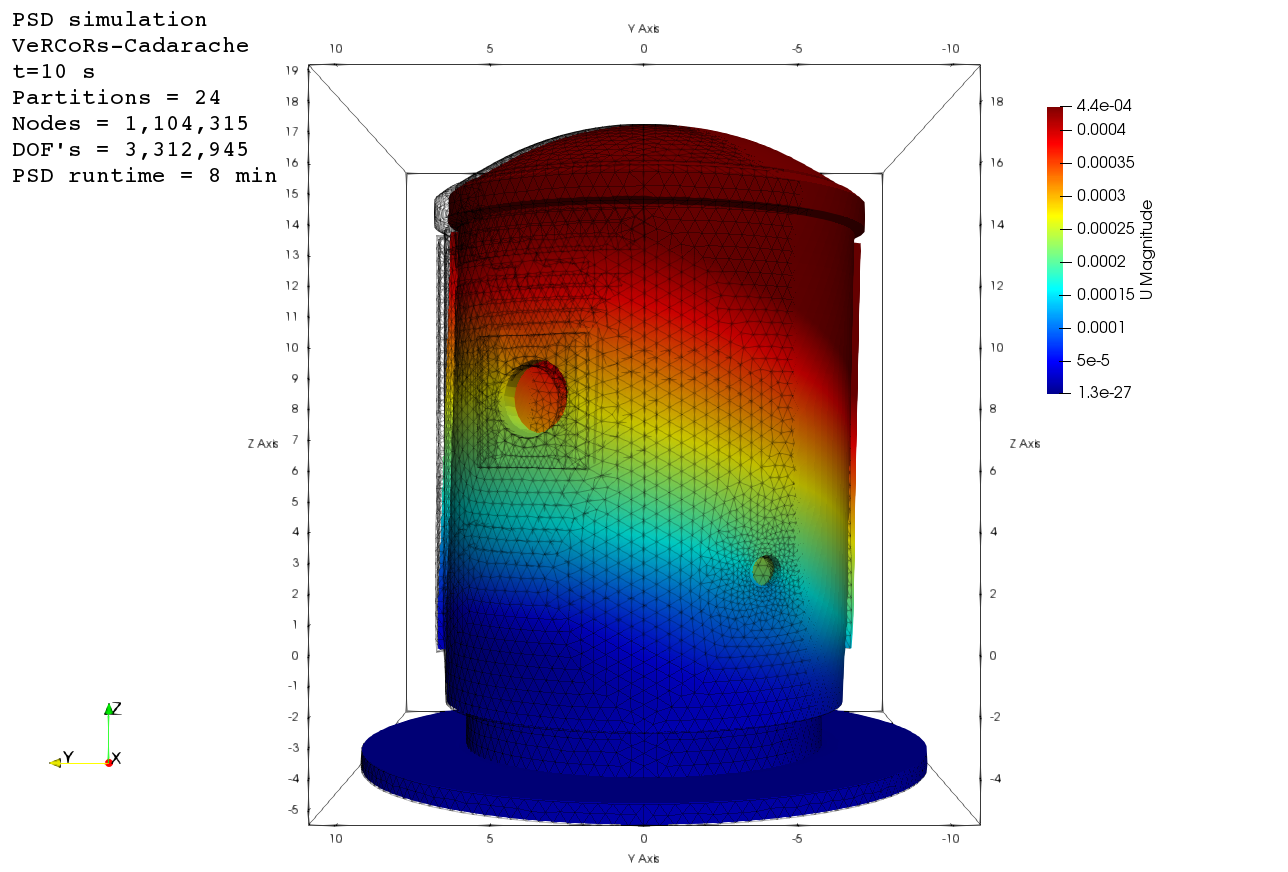
\includegraphics[width=0.45\textwidth]{./Images/vercor140.png}	
	\caption{Seismic signal on vercor nuclear building.}
	\label{fig:vercor-sesimic}
\end{figure}

\begin{figure}
	\centering
	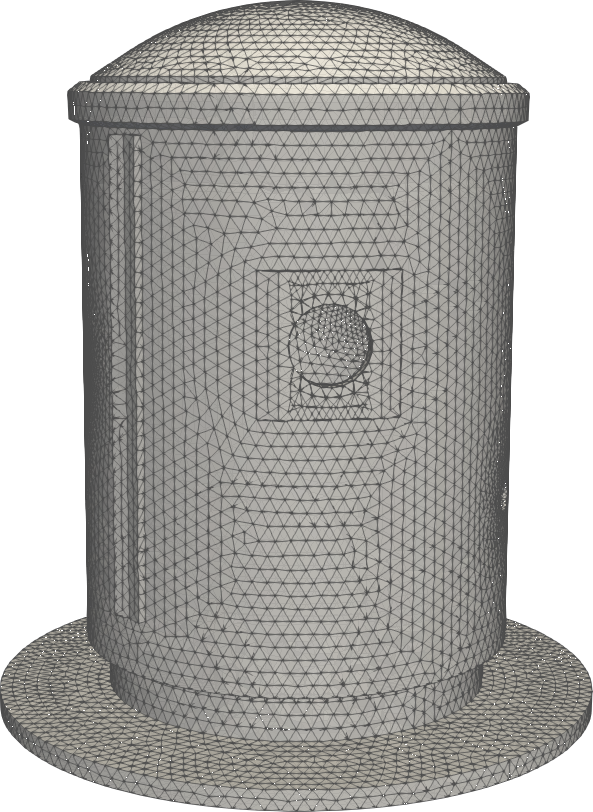
\includegraphics[width=0.32\textwidth]{./Images/vercor-mesh-trans.png}        
	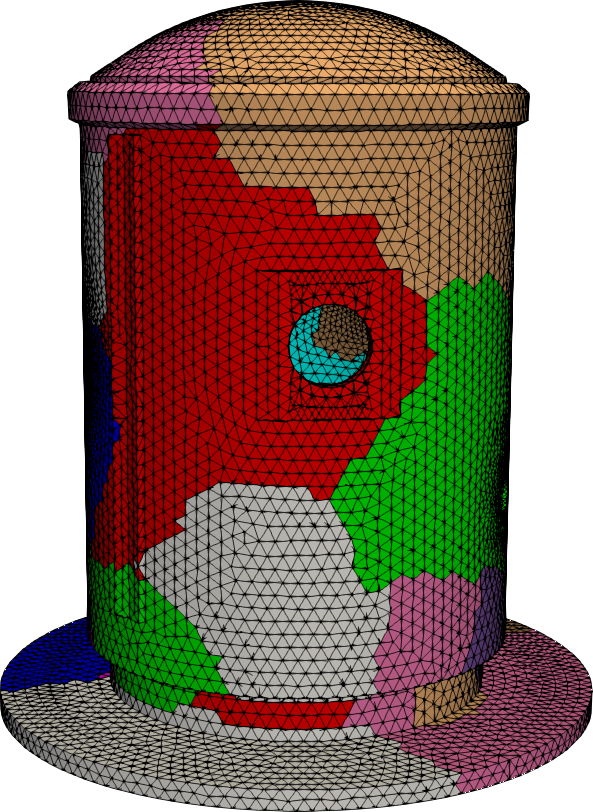
\includegraphics[width=0.32\textwidth]{./Images/vercor-part-trans.png}    
	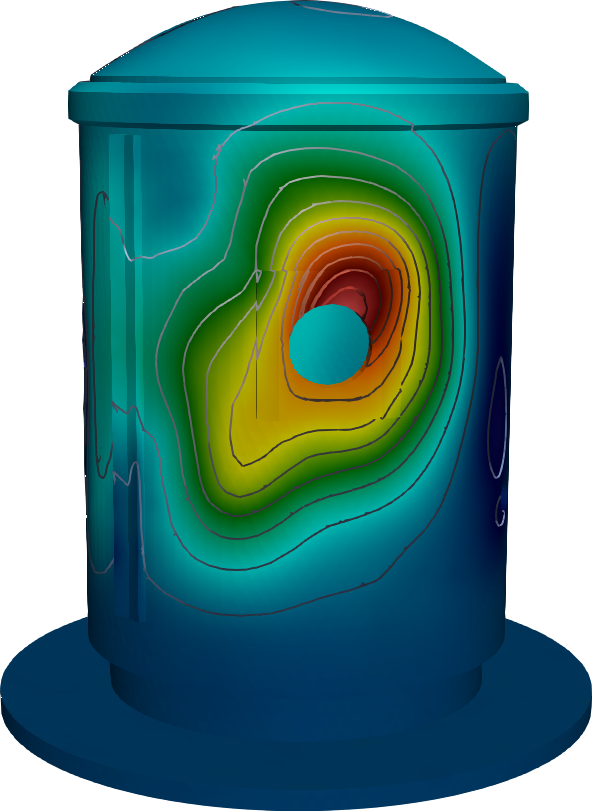
\includegraphics[width=0.32\textwidth]{./Images/vercor-cont-trans.png}
	\caption{Damage mechanics of vercor nuclear building.}
	\label{fig:vercor-damage}
\end{figure}